\documentclass[a4paper, 11pt, oneside, polutonikogreek, french]{article}
\usepackage{kmath, kerkis}
\usepackage[T1]{fontenc}
\usepackage{textalpha}
\usepackage{graphicx}
\usepackage{float}
\usepackage{lscape}
\graphicspath{ {./} }
\usepackage[figurename=]{caption}
\usepackage{listings}
\usepackage{subcaption}
\lstset{basicstyle=\ttfamily}
\usepackage{wasysym}
% Babel package:
\usepackage{babel}
\usepackage{cjhebrew}
% With XeTeX/LuaTeX, load fontspec after babel to use Unicode
% fonts for Latin script and LGR for Greek:
\ifdefined\luatexversion \usepackage{fontspec}\fi
\ifdefined\XeTeXrevision \usepackage{fontspec}\fi

% "`Lipsiakos" italic font `cbleipzig`:
\newcommand*{\lishape}{\fontencoding{LGR}\fontfamily{cmr}%
		       \fontshape{li}\selectfont}
\DeclareTextFontCommand{\textli}{\lishape}
\usepackage{tocloft}
\cftsetindents{subsubsection}{3em}{7em}
\cftsetindents{subsection}{3em}{6em}
\cftsetindents{section}{3em}{6em}
\usepackage[dvipsnames]{xcolor}
\usepackage{eso-pic,graphicx}
\usepackage[top=28mm, bottom=28mm, outer=23mm, inner=160mm, landscape]{geometry}
\setlength{\columnsep}{70pt}
\color{Black}
\AddToShipoutPictureBG{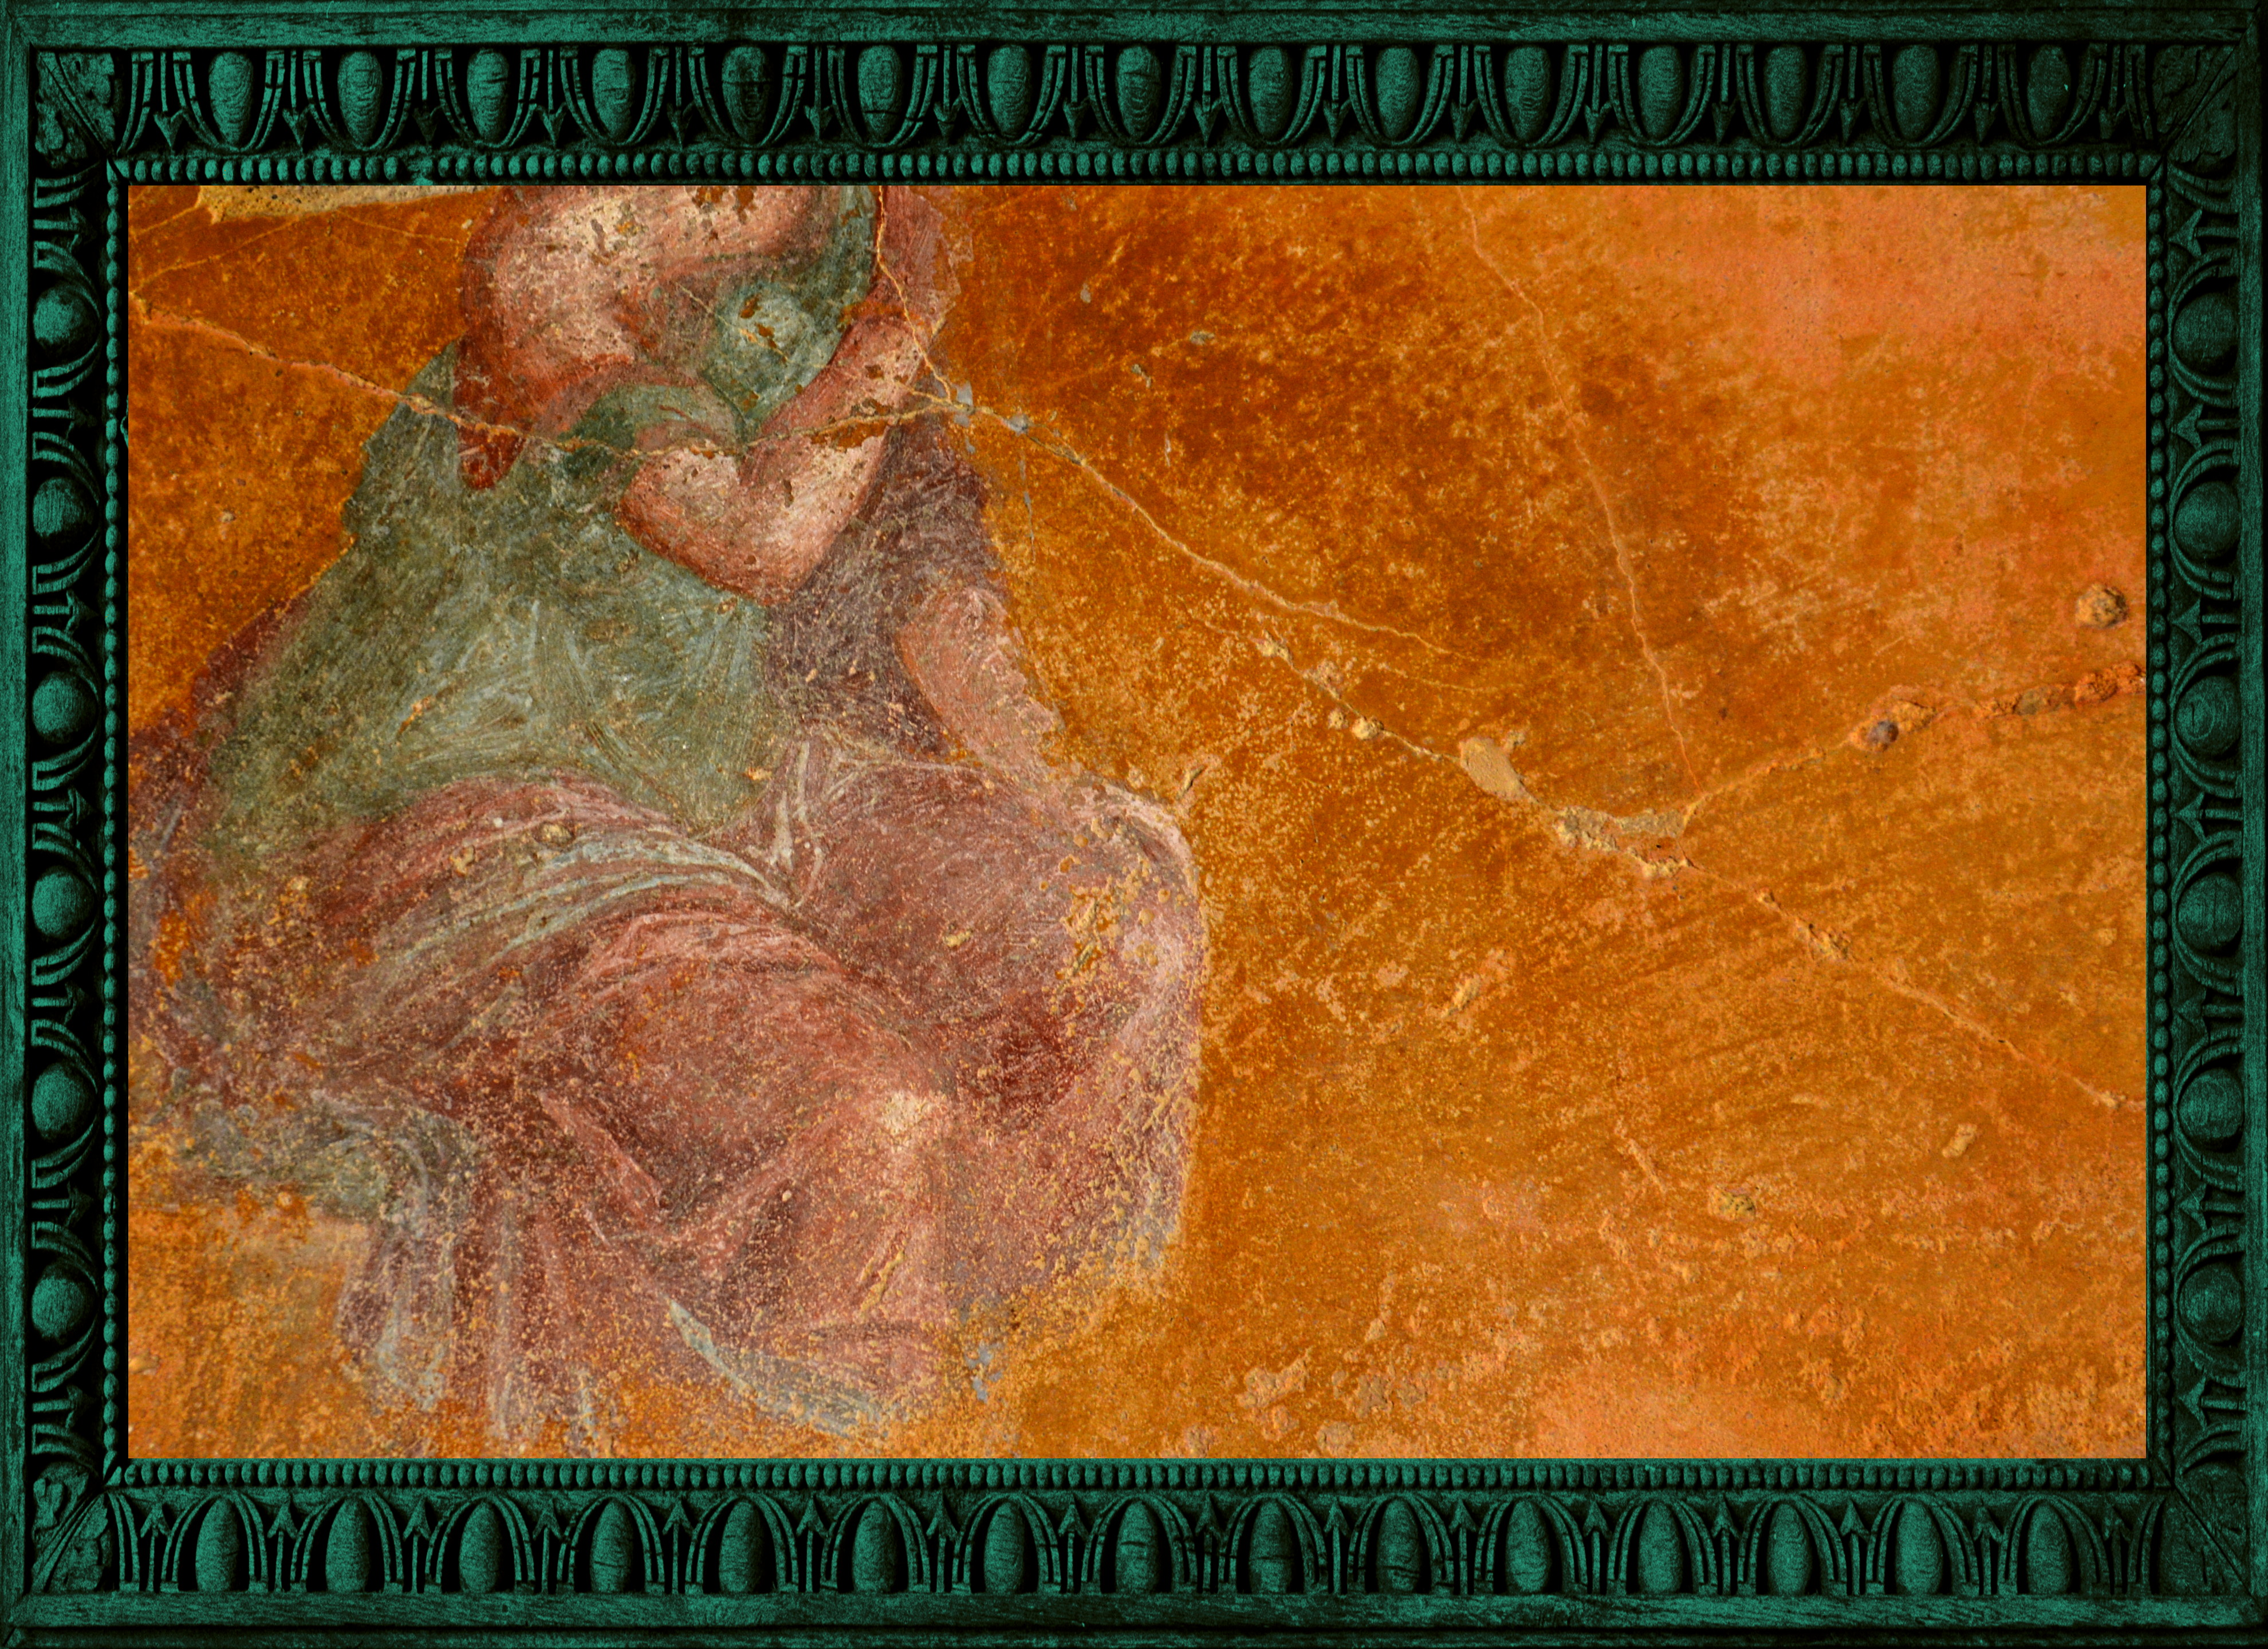
\includegraphics[width=\paperwidth,height=\paperheight]{angerona.jpeg}}
\usepackage{booktabs}
\setlength{\emergencystretch}{15pt}
\usepackage{microtype}
\usepackage{fancyhdr}
\begin{document}
\bfseries
\renewcommand\thefootnote{\bfseries{\arabic{footnote}}}
\let\oldfootnote\footnote
    \renewcommand{\footnote}[1]{\oldfootnote{\bfseries#1}}
\begin{titlepage} % Suppresses headers and footers on the title page
	\centering % Centre everything on the title page
	%\scshape % Use small caps for all text on the title page

	%------------------------------------------------
	%	Title
	%------------------------------------------------
	
	\rule{\textwidth}{1.6pt}\vspace*{-\baselineskip}\vspace*{2pt} % Thick horizontal rule
	\rule{\textwidth}{0.4pt} % Thin horizontal rule
	
	{\scshape\small Description d'une Pierre gravée}
	
	{\scshape\normalsize avec des Recherches sur \\\LARGE les Divalia et les Angeronalia \\\LARGE des Romains}
	
	{\scshape\small comme Culte secret de Vénus Genitrix}
	
	\rule{\textwidth}{0.4pt}\vspace*{-\baselineskip}\vspace{3.2pt} % Thin horizontal rule
	\rule{\textwidth}{1.6pt} % Thick horizontal rule

	%------------------------------------------------
	%	Subtitle
	%------------------------------------------------
	

	\vspace{1\baselineskip}
	
	{\scshape Par \Large M. Jules Sichel} % Subtitle or further description
	
    
    %------------------------------------------------
	%	Cover photo
	%------------------------------------------------
	
	
	%------------------------------------------------
	%	Editor(s)
	%------------------------------------------------
    \vspace*{\fill}

	\vspace{1\baselineskip}

	{\small\scshape Extrait de \emph{Revue Archéologique}, 2\textsuperscript{e} et 3\textsuperscript{e} année}
	
	{\small\scshape{Paris, 1846}}
	
	\vspace{0.5\baselineskip} % Whitespace after the title block

    \scshape Solar Anamnesis Edition  % Publication year
	
	{\scshape\small CC0 1.0 Universal} % Publisher
\end{titlepage}
\setlength{\parskip}{1mm plus1mm minus1mm}
\setcounter{tocdepth}{3}
\setcounter{secnumdepth}{3}
\large
\tableofcontents
\clearpage
\listoffigures
\clearpage
\section{Première Partie}
\subsection{Première Article}
\begin{figure}[H]
\centering
\includegraphics[width=0.25\textwidth,keepaspectratio]{figures/fig01-trans.png}
\caption{\bfseries Pierre gravée.}
\end{figure}
\paragraph{}
M. Champollion-Figeac, l'un des conservateurs de la Bibliothèque royale, informé par moi que je m'occupais de recherches sur des pierres sigillaires d'oculistes romains, a eu l'obligeance de me communiquer un cachet antique. Cette pierre qui fait partie de sa collection n'est pas un cachet d'oculiste. De prime abord, sa forme et la matière dans laquelle il a été taillé le prouvent. Les pierres sigillaires d'oculistes romains sont quadrangulaires et le plus souvent en serpentine ou en stéatite verte, quelquefois en une espèce de pierre semblable brunâtre. Le cachet en question, au contraire, est en silex calcédoine brûlé, d'une couleur jaunâtre, ayant dans la plus grande partie de sa surface une teinte jaune blanchâtre, due à l'action du feu. Il représente la moitié d'un ovoïde, dont la convexité, qui, du côté de la face gravée, n'est sensible qu'à la circonférence, est extrêmement marquée du côté opposé, ce qui donne à ce cachet une épaisseur de presque 15 millimètres. Sur sa face aplatie, dont nous donnons ici la copie exacte, il est long de 35 et large de 23 millimètres environ ; c'est sur le pourtour de cette même face qu'on peut lire gravé \emph{en lettres renversées} de 2 millimètres et demi de hauteur : PVBLIVS SEPVLLIVS MACER, sans aucun doute le nom du propriétaire, destiné à être imprimé lisiblement. La moitié inférieure de cette face est occupée par un autel taillé en creux, au milieu duquel est disposé longitudinalement le mot DIVALIA. Ce mot, comme tous les autres qu'on lit encore sur cette face, est gravé en lettres également creuses, mais plus petites et \emph{droites}, de manière à devoir former une empreinte renversée. Sur le côté droit de l'autel, à la gauche de l'observateur, on lit le mot AENEAS, sur son côté gauche IVLVS. Au-dessous de la base de l'autel, dans toute la largeur de la pierre, se trouvent les mots VEN. GENI. Tous les caractères de ces inscriptions sont d'un très-beau travail et on ne peut plus lisibles. Au-dessus et à quelque distance de l'autel se trouve une étoile. Sur l'angle supérieur gauche de l'autel est appuyé le signe astronomique de la terre, ou la croix ansée asiatique, un peu inclinée à gauche ; sur l'angle droit correspondant un \emph{lituus}.

Telle est la description exacte de cette face du cachet. Son explication est simple et n'offre pas de difficulté.

La fête appelée \emph{Divalia}, que les \emph{Fasti calendares} (Gruter. Thes., p. 133) indiquent au 21 décembre, est interprétée généralement comme étant celle de la déesse \emph{Angerona}, qui est représentée dans la position du silence, c'est-à-dire, les doigts appliqués sur la bouche fermée. Les auteurs anciens et modernes ne sont pas d'accord sur le point de savoir quelle est cette divinité et quelles sont ses attributions. Aucun d'eux n'a songé à Vénus, ce qui cependant était bien naturel, d'une part, à cause du nom de \emph{Diva parens}, que Virgile donne plusieurs fois à la mère de l'Amour et d'Énée (Æn. 4., 365 ; 8., 531 ; \emph{diva Venus} 2., 787 ; \emph{diva creatrix} 6., 367 ; DIVAI. VENERI, inscription chez Muratori, 57, 4) ; et d'autre part, parce que les \emph{Divalia} étaient célébrés dans le temple de \emph{Volupia}, déesse de la volupté (\emph{St. Augustin.} Civit. D. 4., 8. \emph{Volupia, quæ a voluptate appellata est. Ib.}, 11. \emph{De voluptate Volupia nuncupatur}). Dans le cachet en question cette signification est mise hors de doute par les mots de \emph{Venus Genitrix} et les noms de ses descendants \emph{Æneas} et \emph{Iulus}. L'attitude d'Angerona et le silence qu'elle recommande, ainsi que son nom obscur et non expliqué, qui n'est pas même écrit d'une manière uniforme par tous les auteurs, puisqu'ils l'appellent tantôt \emph{Angerona}, tantôt \emph{Angeronia}, toutes ces particularités semblent indiquer un culte secret de Vénus. Une autre circonstance rappelle également le secret recommandé aux adeptes : c'est que, dans ce cachet, tout ce qui se rapporte aux rites sacrés est gravé en lettres droites dont l'empreinte renversée offre plus de difficulté à se laisser lire. Il en est de même des symboles placés au-dessus de l'autel ; tout dans le culte d'Angerona annonce le mystère. Il me paraît même permis de croire que cette déesse était l'antique divinité tutélaire de Rome. Le nom intime de cette divinité, ainsi que le véritable nom de la ville éternelle, était un secret d'État, un mystère de religion ; il ne devait être connu et prononcé que par les initiés. Dans sa statue, Angerona est représentée les doigts appliqués sur les lèvres (Macrobe) comme Harpocrate, ou même, d'après Pline, Solin et un autre passage de Macrobe, les lèvres bandées et scellées, afin d'indiquer le profond silence que tout adepte devait observer sur son culte comme étant celui de Vénus, mère de la race énéenne (\emph{Æneadum genitrix} Lucret. 1., 1.) et déesse tutélaire de Rome. Nous appuyons cette opinion d'un côté sur la tradition de la fondation de Rome par les descendants de Vénus et d'Énée, croyance religieuse généralement reçue chez les Romains et pour ainsi dire passée à l'état d'article de foi ; et d'un autre côté nous la faisons reposer plus encore sur les passages suivants tirés des anciens auteurs. Nous les rapportons en entier, à cause de leur importance et parce que, selon nous, ils établissent la preuve que les \emph{Divalia} ou \emph{Angeronalia} étaient la fête de Vénus, déesse tutélaire de Rome, qu'on y adorait sous le nom secret et très-probablement exotique d'Angerona.

Plin. \emph{H. N.} 3., c. 5, s. 9. « Roma ipsa : cujus nomen alterum dicere, arcanis cærimoniarum nefas habetur : optimaque et salutari fide abolitum enuntiavit Valerius Soranus, luitque mox pœnas. Non alienum videtur inserere hoc loco exemplum religionis antiquæ, ob hoc maxime silentium institutæ. Namque Diva Angerona, cui sacrificatur A. D. 12. Kalend. Januarii, ore obligato obsignatoque simulacrum habet. »

Solin. \emph{Polyhist.} c. 1. « Traditur etiam proprium Romæ nomen et verum magis, quod nunquam in vulgum venit, sed vetitum publicari, quandoquidem quo minus enunciaretur cærimoniarum arcana sanxerunt, ut hoc pacto notitiam eius aboleret fides placitæ taciturnitatis. Valerium denique Soranum, quod contra interdictum id eloqui ausus foret, ob meritum profanæ vocis neci datum. Inter antiquissimas sane religiones sacellum colitur Angeronæ, cui sacrificatur ante diem duodecimum Kalendarum Januariarum : quæ diva præsul silentii istius prænexo obsignatoque ore simulacrum habet. »

Macrobe (\emph{Saturnal.} 3., 9), après avoir rapporté que les Romains, lors du siége d'une ville ennemie, avaient l'habitude d'adresser à ses dieux tutélaires des prières, afin de les engager à abandonner la ville assiégée et de venir habiter Rome, continue ainsi : « Propterea ipsi Romani et deum, in cujus tutela urbs Roma est, ut ipsius urbis Latinum nomen ignotum esse voluerunt. Sed dei quidem nomen nonnullis antiquorum licet inter se dissidentium libris insitum : et ideo vetusta persequentibus quicquid de hoc putatur innotuit. Alii enim Jovem crediderunt, alii Lunam : sunt qui Angeronam quæ digito ad os admoto silentium denuntiat. Alii autem, quorum fides mihi videtur firmior, Opem Consiviam esse dixerunt. Ipsius vero urbis nomen etiam doctissimis ignotum est, caventibus Romanis ne, quod sæpe adversus urbes hostium fecisse se noverant, idem ipsi quoque hostili evocatione paterentur, si tutelæ suæ nomen divulgaretur. »

\emph{Id.} (\emph{Saturnal.} 1., 10.) « Duodecimo Kalendas Januarias feriæ sunt Divæ Angeroniæ, cui pontifices in sacello Volupiæ sacrum faciunt : quam Verrius Flaccus Angeroniam dici ait, quod angores ac animorum sollicitudines propitiata depellat. Masurius adjicit simulacrum huius deæ ore obligato atque signato in ara Volupiæ propterea collocatum, quod qui suos dolores anxietatesque dissimulant, perueniant patientiæ beneficio ad maximam voluptatem. Julius Modestus ideo sacrificari huic deæ dicit, quod populus romanus morbo, qui angina dicitur, præmisso voto sit liberatus. »

Festus v. Angeronalia. « Angeronæ deæ sacra a Romanis instituta sunt, quum angina omne genus animalium consumeretur : cuius festa Angeronalia dicebantur. »

Plin. \emph{H. N.} 28., c. 2, s. 4. « Verrius Flaccus auctores ponit, quibus credat, in oppugnationibus ante omnia solitum a Romanis sacerdotibus evocari deum, cujus in tutela id oppidum esset : promittique illi eundem aut ampliorem apud Romanos cultum. Et durat in pontificum disciplina id sacrum : constatque ideo occultatum, in cujus dei tutela Roma esset, ne qui hostium simili modo agerent. »

Plutarque (\emph{Quæst. Roman.} p. 278), en parlant de cette même superstition, ajoute qu'il était non-seulement défendu de prononcer ce nom de cette divinité tutélaire de Rome, mais encore de dire ou de chercher à savoir (ζητεῖν), quel était son sexe. Il mentionne aussi la punition de Valerius Soranus.

Varro, De lingua lat., l. 4., p. 46, ed Bip. « Intra muros altera porta Romanula, quæ est dicta ab Roma ; quæ habet gradus in navalia ad Volupiæ sacellum. »

\emph{Id., ib.}, l. 5., p. 58. « Angeronalia ab Angerona, cui sacrificium fit in curia. »

Orell. Inscrr. 2., p. 410. \emph{Verrii Flacci fasti prænestini}, Decemb. 21. « Feriæ divales Angeroniæ, cui sacrificium in ara Volupiæ fit. »

A des passages aussi explicites, il me reste peu de chose à ajouter. \emph{Angerona}, bien loin de venir d'\emph{angere}, d'\emph{angina} ou de toute autre racine latine, me semble d'origine asiatique. C'est probablement le nom de quelque Vénus orientale, comme \emph{l'Astarte} ou \emph{l'Astaroth} des Syriens ou la Mylitta des Assyriens. Déesse tutélaire de la race énéenne, elle est probablement venue avec elle lors de son émigration après le sac de Troie. Peut-être même sont-ce là ces dieux Pénates (\emph{cape sacra manu, patriosque Penates}, Æn., 2., 717 ; \emph{sacra suosque tibi commendat Troja Penates}, ib. 293 ; \emph{Dî, precor, Æneæ comites}, Ov. Métam. 15., 861) qu'Énée, avant de songer à emporter toute autre chose, a si pieusement sauvés du pillage et de l'incendie. Il était on ne peut plus naturel qu'Énée et ses descendants fissent présider cette divinité de leur patrie (\emph{patriique Penates}, Æn., \emph{loc. cit.} ; \emph{Dî patrii indigetes} Georg. 1., 498) à la fondation et aux destinées de Rome.

C'est par cette raison sans doute qu'on voit sur des monnaies de César, destinées à rappeler ces circonstances et le culte de Vénus (\emph{Goltz.} Nomism. Cæsaris, 6., 1-3, 2., 24. \emph{Morell.} Fam. rom. numism., Jul. 1., V et M. \emph{Riccio}, Monete delle famiglie di Roma 22., Julia 8), l'image de cette déesse, et sur le revers celle d'Énée portant sur le dos son père Anchise et dans la main ses dieux Pénates, dieux qui sont représentés sous la figure d'une petite statuette de Vénus Victrix ailée et le casque en tête, mais surtout reconnaissable par un bouclier dont plusieurs cercles concentriques entourent la circonférence, bouclier tout à fait identique à celui que porte cette Vénus (\emph{Goltz.} 7., 13 et 17. \emph{Mor.} Sepull. 3. \emph{Ricc.} 43., Sepull., 2, 3). Je n'ignore pas que dans cette figurine on a voulu voir le Palladium. Ce n'est pas sans surprise que je trouve Heine (Excurs. 9. ad Æneid, 2., p. 344 et 346, ed. 3.) au nombre de ceux qui ont adopté cette opinion, selon moi difficile à justifier. Car il n'est dit nulle part d'une manière positive que cette image de Minerve, déjà enlevée par Ulysse et Diomède avant la chûte d'Ilium, ait été rapportée par Énée. Les traditions, au contraire, sont presque unanimes pour affirmer que son premier soin fut de mettre en sureté ses dieux Pénates. D'ailleurs, c'est un point sur lequel nous reviendrons. D'un autre côté, Vénus Victrix et Vénus Genitrix, comme nous espérons le prouver plus loin, sont identiques et dérivent toutes les deux de cette Vénus orientale apportée en Italie par les Énéades. Son culte pourrait avoir pris naissance et avoir été secrètement pratiqué d'abord en Lydie. Ou bien encore le vrai nom de cette divinité, devenue la déesse tutélaire de Rome, pourrait avoir été enveloppé de mystère par les premiers Romains, leurs gouvernants ou leurs prêtres, dominés qu'ils étaient par la superstition religieuse que racontent Macrobe et Pline. Ce qui tendrait à nous confirmer dans cette opinion, c'est que chez les anciens Romains, comme le rapporte Macrobe (\emph{Saturn.} 1., 12), le nom grec et latin de Vénus n'existait pas ; cela forme un contraste frappant avec la croyance si répandue parmi les Romains, qui faisait remonter leur origine à cette déesse. « \emph{Sed ne in carminibus quidem Saliorum Veneris ulla, ut ceterorum cælestium, laus celebratur. Cincio etiam Varro consentit affirmans nomen Veneris ne sub regibus quidem apud Romanos vel latinum vel græcum fuisse.} » Ce passage encore nous paraît prouver que le culte de Vénus, importé de l'Orient avec les descendants d'Énée, s'adressait à cette déesse sous un nom qu'on tenait secret afin de donner le change sur la véritable religion de l'État. Plus tard seulement on y substitua ceux de Vénus, d'Angeronia et de Volupia, en s'arrangeant toutefois de façon à ce qu'on ne découvrît pas l'identité mystérieuse de ces divinités. Pour rendre ce secret impénétrable et empêcher la profanation d'un nom d'où dépendait le salut de l'État, les Romains avaient pris des mesures sévères et terribles, témoin l'exécution sanglante de l'imprudent Valerius, racontée par Pline et Solin. Ils n'en avaient pas moins consacré à cette divinité des fêtes publiques sous le nom des \emph{Angeronalia}, qu'ils célébraient à Angerona ou Angeronia, dans le temple de Volupia, autre nom de Vénus. Comme Festus, Macrobe, etc., ignoraient le culte secret de cette déesse, rien d'étonnant qu'on ait cherché à la définir de manières si diverses. Les uns font dériver son nom de \emph{angere}, les autres de \emph{angina}. Scaliger (\emph{ad Varr.} 5., p. 58) voulut même, par une transposition (\emph{Angenora} pour \emph{Angerona}), le faire venir de \emph{angere ora}, à cause de la manière dont elle était représentée dans sa statue, qui avait du rapport avec celle du dieu du silence. Pour moi, bien que je ne me pique pas d'être grand étymologiste ni très-fort sur les langues orientales, je ne puis m'empêcher de trouver un rapport d'assonance entre les mots \emph{Astaroth} et \emph{Angerone}. Or, \emph{Astaroth} ou « \emph{Aschtoreth}, divinité de Sidon, » (1. Reg., 11, 5) est le nom donné par la Bible à \emph{Astarte} que Cicéron (de \emph{Nat. Deor.}, 3., 23) déclare être une Vénus syriaque. On trouve aussi (Goltz. August. nomism., 10., 116, 54., 17 ; Thesaur. Morell., ed. Wessel., August. t. 40., 25) une monnaie ayant d'un côté la tête d'Auguste et de l'autre celle de Vénus Genitrix, avec l'inscription : ΘΕΑΣ ΣΙΔΩΝΟΣ. D'après Hérodote (1., 131) Vénus Uranie était adorée chez les Assyriens sous le nom de Mylitta, chez les Arabes sous le nom d'Alitta (lisez : comme 3., 8, \emph{Alilat}, la nuit, le ciel étoilé). A Ascalon, en Syrie, elle avait, selon le même auteur (1., 105), son temple le plus ancien. Au dire des Cypriotes eux-mêmes, le temple qu'elle avait à Chypre tirait son origine de la Syrie (ἐντεῦθεν ἐγένετο), ce qui est fort important pour l'explication de l'un des symboles gravés sur le cachet de Sepullius. Le temple de Cythère avait été fondé aussi par des Phéniciens, natifs (ἐόντες) de cette même Syrie. On pourrait probablement poursuivre plus loin cette connexité du culte d'Angerona et d'une Vénus orientale ou phénicienne. Peut-être même ces recherches ont-elles déjà été faites, car il est souvent question de cette Vénus phénicienne chez les mythologues anciens et modernes. Pour moi, il m'est impossible, dans ce moment, de donner plus de développement à cette idée et d'examiner si elle a été traitée, et de quelle manière, par les auteurs qui m'ont précédé. La croix ansée asiatique, ajoutée comme symbole sur le cachet, me semble donner plus de vraisemblance à cette conjecture. J'abandonne sur ce point toute espèce de recherches ultérieures aux savants qui se sont spécialement occupés de la mythologie et de la philologie orientales. Festus et Modestus, à la vérité, pour justifier l'étymologie qu'ils établissent, prétendent que le nom avait été imposé à la déesse après qu'elle eut sauvé les Romains dans une épidémie d'angine, sans doute d'esquinancie gangréneuse, qui n'épargnait pas même les animaux ; mais cette particularité ne fournit qu'un argument extrêmement contestable. Car les Romains, après avoir eu vainement recours ou même avant de s'être adressés aux autres dieux, pouvaient fort bien avoir invoqué cette déesse justement par l'effet d'une ressemblance fortuite entre \emph{Angina} et \emph{Angerona}, et à cause du sens supposé de ce dernier mot. Sa vraie signification, ainsi que les attributions réelles de cette divinité, devaient nécessairement leur échapper.

Le nom lui-même et les autres circonstances que nous avons passées en revue nous semblent apporter de fortes présomptions en faveur de l'idée que nous avons adoptée, surtout d'après les inscriptions et les symboles que présente le cachet de Sepullius. Angerona, d'après son sens véritable et profond, est pour nous une Vénus d'origine orientale, devenue déesse nationale et tutélaire de Rome. Plus tard, après l'érection du temple de Vénus Genitrix, son culte y fut solennellement, mais mystérieusement célébré, comme le prouve la pierre gravée inédite qui fait le point de départ de nos recherches. Jusqu'à cette époque il avait été relégué, et depuis il fut continué ostensiblement, dans une chapelle d'un extérieur modeste (\emph{Volupiæ sacellum}, Varr., Macrob., \emph{sacellum Angeronæ}, Solin), dans le même but de superstition religieuse, pour ne pas attirer par trop de faste l'attention des profanes et surtout des ennemis, de peur qu'arrivant à reconnaître le vrai nom de la déesse, ils ne l'entraînassent loin de la ville. Voilà pourquoi, même au temps de toute la force et de toute la grandeur de Rome, après que le temple de Vénus Genitrix fut achevé, le nom d'Angeronia ne parut point dans les solennités publiques, ni même sur les insignes des adeptes. Par cette raison, il ne figure pas sur le cachet de Sepullius, prêtre de la déesse ; bien plus, le mot Divalia y est tracé en lettres droites, afin de ne point frapper les yeux du profane vulgaire par une empreinte trop lisible et de ne point reporter la pensée vers l'identité d'Angeronia avec Vénus, protectrice de Rome.

Maintenant que nous avons essayé d'expliquer les inscriptions qui ont un rapport direct avec les mystères religieux eux-mêmes, et qui pour cela sont gravées en lettres droites, destinées par conséquent à former une empreinte renversée et difficilement lisible, passons aux symboles qu'on voit au-dessus de l'autel, et voyons s'ils prêtent à une interprétation qui, sans être forcée, invraisemblable, soit en harmonie avec le sens que nous venons de trouver dans les mots inscrits sur l'autel et autour de lui.

D'abord, l'étoile nous reporte tout naturellement à celle de Vénus (\emph{Hesperus}), d'après ce que nous venons de dire sur l'identité de cette déesse et d'Angerone. C'est là une interprétation qui se présente d'elle-même à l'esprit. On voit une étoile semblable au-dessus de la tête de \emph{César Imperator}, sur une de ses monnaies (Goltz. Cæs. 1., 1. Mor. Jul. 2., 4. Ricc. 23., 21). Ce symbole doit exprimer sa filiation avec la déesse, ce dont nous aurons besoin de parler avec quelques détails dans le cours de cette dissertation. L'étoile de Vénus se voit fréquemment sur des monuments qui se rattachent de près ou de loin à son culte. On ne doit pas être étonné de la voir sur des monnaies au-dessus de l'image de Vénus Victrix (Goltz. Cæs. 10., 2), ou de celle de César déifié (Mor. Jul. 8., 50. ; Goltz. Cæs. 4., 44, 46-48. 23., 5. 33., 7 et 9, \emph{et passim}), et d'Auguste avec l'épithète \emph{Divi Filius} (Goltz. Aug. 27, 1 et 3).

Mais souvent même on rencontre cette étoile dans des circonstances qui ne font aucune allusion au culte de Vénus, ni à la famille julienne, de manière à faire croire, comme nous l'avons déjà dit, que Vénus était regardée comme étant liée intimement aux affaires de la république et aux destinées de Rome. C'est ainsi qu'elle se trouve sur des monnaies de Marc-Antoine (\emph{Id.} Cæs. 33., 7, 9 \emph{et passim}). En général, on trouve ce symbole joint aux noms de personnages qui ont rempli les fonctions de grand pontife et d'augure. Ce qui, du reste, rend plus probable qu'il s'agit bien là de Vénus, et que le culte de cette déesse jouait un grand rôle chez les Romains dans tout ce qui concernait les usages sacrés et la religion, c'est une monnaie de Marc-Antoine (\emph{Ib.} 35., 12), avec l'inscription : M. ANTON. M. F. M. N. AUG. IMP. TER. On y voit un autel ou trépied, présentant d'un côté le \emph{lituus}, de l'autre côté le \emph{simpulum} ou \emph{simpuvium}, et au-dessus la même étoile. Entre les trois pieds de l'autel sont placés deux oiseaux d'une taille fort petite, soit les tourterelles, soit les moineaux consacrés à la déesse de l'amour. C'est du moins ainsi que je crois devoir les interpréter, autant à cause de leur petitesse et de leur nombre double, que pour la manière dont ils sont perchés, qui ne rappelle en rien les oiseaux destinés à l'auspicium. Sur les monnaies frappées par des augures, cette dignité n'a d'ordinaire pour attribut qu'un seul oiseau qui en outre est plus grand, placé à terre et presque toujours facilement reconnaissable pour un coq. Il en est au moins ainsi dans les figures données par Goltz, qui, étant pour la plupart notablement grossies, admettent des détails qu'on cherche en vain chez Morell et Riccio. Sur une seule médaille de Lepide, grand pontife (Goltz. Cæs. 21., 15, et 27., 1), on voit deux oiseaux plus grands, mais qui évidemment, par leur forme et leur attitude, représentent deux individus du genre des gallinacés, coqs ou poules, au moment de prendre leur nourriture, ce qui désigne clairement un attribut de l'augurat. On sait que les augures puisaient leurs présages surtout dans le plus ou moins d'avidité avec laquelle ces animaux mangeaient. Pour en revenir à la médaille de Marc-Antoine, elle me semble prouver le rôle important que Vénus jouait dans les cérémonies religieuses de Rome ; d'ailleurs, cette médaille méritait d'être mentionnée, à cause de son analogie avec le cachet de Sepullius. Nous avons aussi trouvé une monnaie d'Auguste semblable (Goltz. Aug. 27., 1), sur laquelle est figuré un autel ou trépied surmonté de deux étoiles, et présentant sur le côté un lituus. Une autre monnaie encore (\emph{Id.} Cæs. 22., 5) nous paraît digne de remarque. Son revers porte au milieu la même étoile ; mais cette étoile est de plus grande dimension, et en outre entourée d'ornements disposés en forme de cercle, autour duquel on lit : M. AIMIL. M. F. Q. N. LEPIDVS. PRAEF. VRB. Dans cette occasion, il s'agit d'un fonctionnaire étranger à la famille julienne, n'étant revêtu d'aucune dignité sacerdotale, mais chargé de fonctions administratives suprêmes. Ici l'étoile de Vénus doit faire allusion à cette divinité tutélaire de la ville des sept collines, divinité enveloppée de mystère, que nous croyons Vénus Genitrix, origine de la race énéenne par qui Rome fut fondée ; en un mot, cette déesse qui, selon nous, était adorée sous le nom d'\emph{Angeronia}. Cette supposition nous paraît gagner en vraisemblance, si l'on considère la face de cette même médaille\footnote{Nous employons indistinctement les mots \emph{médailles} et \emph{monnaies}, n'ayant pas eu le temps de rechercher chaque fois s'il s'agissait des unes ou des autres, ce qui d'ailleurs, pour notre sujet, était parfaitement indifférent.} (22., 2). Elle porte la tête de la déesse Rome, coiffée de ce même casque que nous avons vu à Vénus Victrix, avec la légende : ROMA.

Pour le cachet qui fait le sujet de cette dissertation, on pourrait donc, à la rigueur, se borner à voir dans l'étoile celle de Vénus, et l'explication que nous avons donnée de l'ensemble n'en souffrirait pas. Mais elle est insuffisante, par les motifs que nous exposerons dans la prochaine livraison.
\subsection{Deuxième Article}
\paragraph{}
Loin d'être une étoile simple, comme dans les monnaies et les médailles, celle qui se trouve au-dessus de l'autel, et qui est très-bien gravée comme le reste du cachet de Sépullius, présente une particularité remarquable, particularité qui ne se rencontre pas dans l'effigie habituelle d'Hesperus. Entre les branches de cet astre et dans son diamètre vertical, on voit des points semblables à des étincelles (\emph{lemnisci} dans le passage de Servius que nous citerons). Ils sont assez régulièrement rangés en forme de rayons qui s'étendent de haut en bas, et dans la partie supérieure leur nombre est plus grand. On ne peut méconnaître que cette modification donne à cette figure l'aspect d'une comète. Cette circonstance m'a conduit à penser qu'il s'agit dans l'espèce de la comète de César ; ce qui tendrait à prouver, qu'après la mort du rival de Pompée on a confondu en un seul le culte de Divus Julius et de Venus Genitrix, à laquelle il avait le premier consacré un temple. Les anciens auteurs, dont nous faisons suivre les passages, racontent que, lors des jeux publics célébrés par Auguste en l'honneur de Venus Genitrix et de César placé au rang des dieux, une comète apparut dans le ciel, et que par cette raison l'image de César fut représentée avec une étoile au-dessus de la tête.

\emph{Sueton. Cæs.}, c. 88. « Ludis, quos primo consecratos ei heres Augustus edebat, stella crinita per septem dies continuos fulsit, exoriens circa undecimam horam : creditumque est animam esse Cæsaris in cœlum recepti : et hac de causa simulacro ejus in vertice additur stella. »

\emph{Senec. Natural. quæst.} 7., 17. « Cometes ... qui post necem Divi Julii, Veneris ludis Genetricis, circa undecimam horam diei emersit. »

\emph{Plin.} 1., c. 24 et 25, s. 23. « Cometes in uno totius orbis loco colitur in templo Romæ, admodum faustus Divo Augusto judicatus ab ipso : qui incipiente eo apparuit ludis, quos faciebat Veneri Genitrici, non multo post obitum patris Cæsaris, in collegio ab eo instituto. Namque his verbis id gaudium prodidit : (Iis ipsis ludorum meorum diebus, sidus crinitum per septem dies in regione cœli, quæ sub Septemtrionibus est, conspectum. Id oriebatur circa undecimam horam diei, clarumque et omnibus e terris conspicuum fuit. Eo sidere significari vulgus credidit, Cæsaris animam inter deorum immortalium numina receptam, quo nomine id insigne simulacro capitis ejus, quod mox in foro consecravimus, adjectum est.) Hæc ille in publicum, interiore gaudio sibi illum natum, seque in eo nasci interpretatus est : et, si verum fatemur, salutare id terris fuit. »

\emph{Jul. Obsequens}, c. 128. « Ludis Veneris Genitricis, quos pro collegio fecit, stella hora undecima crinita sub Septemtrionis sidere exorta convertit omnium oculos. Quod sidus, quia ludis Veneris apparuit, Divo Julio insigne capitis consecrari placuit. »

\emph{Serv. ad Virg. Ecl.} 9., 47 : \emph{Ecce Dionæi processit Cæsaris astrum.} « Cum Augustus Cæsar ludos funebres patri celebraret, dic medio stella apparuit : ille eam esse confirmavit parentis sui ... Bæbius Macer circa horam octavam stellam amplissimam quasi lemniscis coronatam, ortam dicit ... Ipse (Augustus) animam patris sui esse voluit, eique in Capitolio statuam super caput auream stellam habentem posuit. Inscriptum in basi fuit : \emph{Cæsari Emitheo}. Sed Vulcatius aruspex in concione dixit, cometen esse qui significaret. ... Hoc etiam Augustus in libro secundo de memoria vitæ suæ complexus est. »

Dio Cassius, qui raconte à peu près la même chose que les auteurs que nous venons de citer, ajoute qu'en raison de l'apparition de cet astre, qui fut regardée comme un prodige, Octavien érigea, dans le temple de Vénus, la statue de César en airain avec une étoile au-dessus de la tête.\footnote{\emph{Dio Cass.} 45., 7. Χαλκοῦν αὐτὸν ἐς τὸ Ἀφροδίσιον, ἀστέρα ὑπὲρ τῆς κεφαλῆς ἔχοντα, ἔστησεν.}

Toutes ces circonstances, et surtout l'adoration de la comète mentionnée par Pline, me font croire que le culte de Venus Genitrix et de Jules César divinisé ne formèrent plus tard qu'un seul, et que la comète gravée sur notre cachet en est un symbole. C'est elle dont parlent Virgile\footnote{Ecl. 9., 47 : \emph{Ecce Dionæi processit Cæsaris astrum}.} et Horace.\footnote{1., carm. 12, v. 46 :\\\hspace*{10mm}\emph{Micat inter omnes}\\\hspace*{10mm}\emph{Julium sidus, velut inter ignes}\\\hspace*{10mm}\emph{Luna minores}.} Je sais que les commentateurs modernes expliquent ces vers autrement ; mais l'allusion à la comète de César me paraît trop claire pour abandonner l'opinion des scoliastes Porphyrion et Acron. Le premier dit : \emph{C. Cæsaris stellam dicit}. Le second cite seulement le vers de Virgile, en le faisant précéder des mots : \emph{Ut Virgilius}. La brièveté de ces annotations indique elle-même que cette croyance, généralement accréditée, faisait autorité et rendait inutiles des explications plus détaillées.

Si nous joignons aux considérations précédentes les monnaies de la famille julienne, où le nom de César est accompagné d'une comète, il ne nous semble plus y avoir aucun doute au sujet de l'explication que nous avons donnée de ce signe. Quant à ces monnaies sur lesquelles nous nous appuyons, on en peut voir un grand nombre dans les différentes collections. La Bibliothèque royale en possède aussi plusieurs ; nous avons cru devoir en faire représenter une des mieux conservées.

\begin{figure}[H]
\centering
\includegraphics[width=0.25\textwidth,keepaspectratio]{figures/fig02-trans.png}
\caption{\bfseries \emph{Divus Iulius.}}
\end{figure}
\paragraph{}
Elle porte la tête laurée d'Auguste tournée à gauche, et sur le revers la comète avec la légende \emph{Divus Iulius}. La queue de la comète est dirigée en haut ; cette circonstance, ainsi que le plus grand nombre d'étincelles (\emph{lemnisci}, Serv.) réunies autour de la partie supérieure de l'étoile dans la pierre gravée de la collection de M. Champollion, s'explique par le passage suivant de Pline\footnote{2., c. 25, s. 22.} : « Cometas Græci vocant, nostri crinitas, horrentes crine sanguineo et comarum modo \emph{in vertice} hispidas. Iidem pogonias, quibus inferiore ex parte in speciem barbæ longæ promittitur juba. » Il en résulte que les anciens donnaient aux comètes différents noms, suivant la direction de leur crinière. L'astre de César avait la sienne dirigée en haut. D'après quelques auteurs ce serait le même que les mages aperçurent en Orient, comme un signe précurseur de la naissance du Christ ; mais cette opinion est en opposition avec les paroles de Pline,\footnote{Loc. cit. : \emph{Incipiente Augusto, non multo post obitum patris Cæsaris}.} d'après lesquelles on ne peut douter que l'apparition de ce phénomène céleste ne soit antérieure de plus de quarante ans à l'ère chrétienne. Cette époque est d'ailleurs fixée d'une manière plus précise par l'indication que fournissent Pline, Suétone, Dio Cassius et Jul. Obsequens. La comète, disent-ils, s'est montrée aux jeux célébrés par Auguste à Venus Genitrix, jeux qui ont eu lieu l'an de Rome 710 ou l'an 44 ayant J. C., l'année même de la mort de Jules César.

Le second symbole que présente le cachet de Sepullius est le \emph{lituus}, bâton sacré trop connu pour avoir besoin d'une explication. Bien qu'il fût l'attribut spécial des augures, il figurait néanmoins dans d'autres solennités religieuses et entre les mains de prêtres d'un ordre différent. De là vient qu'on le trouve sur les monnaies de tous ceux qui ont été revêtus de la dignité pontificale, comme, par exemple, de Jules César, de Lépidus et d'Auguste. Presque toujours ces monnaies portent à côté du nom les mots PONT. MAX. Cet insigne se trouve également sur le revers d'une monnaie d'Auguste\footnote{Goltz. August. 71., 11 ; Morell. Cornel. 2., 7 ; Riccio Cornel. 33.} qui porte cette inscription : LENTULUS FLAMEN MARTIALIS. Ce prêtre est représenté tenant le lituus ; il est donc bien naturel que le bâton augural se retrouve sur le cachet d'un Flamen Divalis, dignité dont Sepullius devait être revêtu.

Il nous reste maintenant à expliquer le dernier symbole. Nous avouerons que sa signification est beaucoup moins facile à découvrir que celle des deux autres. Il est tout à fait semblable au signe astronomique qui, de nos jours, est affecté à notre planète (\earth) ou à celui de Vénus (\venus) renversé, ou encore à la croix ansée asiatique. Du reste, les signes astronomiques dont nous nous servons actuellement remontent, d'après Beckmann,\footnote{\emph{Hist. des Inventions}, 3., 371 et suiv.} aux Grecs et aux Romains. La croix ansée indique un culte de Vénus originaire de l'Orient, où il était très-répandu. Si la tradition de la fondation de Rome par les descendants d'Énée a quelque chose de réel, il n'y aurait rien d'impossible à ce que ce culte eût été importé par eux ; au moins est-ce dans la famille des Énéades qu'il semble avoir été conservé. Quant à la croix ansée, les archéologues savent qu'il y en a un très-grand nombre d'espèces. Celle qui est représentée sur le cachet de Sepullius a une configuration particulière qui se trouve fréquemment, et avec une forme exactement semblable, sur les monnaies de l'île de Cypre ; la croix y est presque toujours tournée en bas. Les cas où la direction de la croix reste douteuse sont en petit nombre. Peut-être que dans les premiers temps cette direction était indifférente, et que par la suite on a varié sa position d'après les circonstances. Selon que la croix regardait en haut ou en bas, le symbole aurait ainsi changé de signification, sans cesser d'appartenir aux mystères de Vénus. Quoi qu'il en soit, depuis les temps les plus reculés cette déesse était adorée à Cypre. Cette île lui était en quelque sorte consacrée ; elle y avait plusieurs temples ; ce qui avait valu à la divine mère d'Énée le nom de \emph{Dea Cypria}. On ne trouvera donc pas extraordinaire si, sans entrer dans d'autres détails que nous interdisent et le manque de temps et nos connaissances imparfaites en archéologie, nous nous bornons à émettre l'opinion que le signe \venus, encore usité de nos jours parmi les astronomes et les chimistes pour représenter Vénus et le cuivre (\emph{cuprum}, appelé d'abord \emph{æs cyprium}), n'est rien autre chose que cette croix ansée asiatique particulière à l'île de Cypre et à son culte de Vénus. Le même signe astronomique, à défaut d'autre, a été renversé pour désigner la terre ; peut-être aussi que ce rapprochement aura été un moyen d'indiquer le peu de distance qui sépare ces deux planètes. La présence de la croix ansée de cette forme particulière sur les monnaies de Cypre\footnote{Cette croix ansée se trouve principalement sur une série de monnaies antiques d'argent dont les légendes en caractères cypriotes n'ont jamais été expliquées. M. le duc de Luynes vient de les lire et va faire paraître, sur ce sujet, comme m'assurent des personnes compétentes, un très-savant et très-intéressant Mémoire. J'espère qu'un grand travail sur la croix ansée, que M. Raoul Rochette publiera prochainement, jettera également une vive lumière sur ce sujet.} est une présomption de plus à nos yeux pour croire que ce culte et ce symbole ont été importés d'Orient. Dans la figure appuyée obliquement sur la gauche de l'autel il est facile de reconnaître cette croix ansée cyprienne, tournée seulement sens dessus dessous et placée ici comme l'un des attributs du culte de Venus Genitrix.

D'après tout ce qui précède et d'après les monnaies de la famille sépullienne, nous nous croyons en droit de conclure que P. Sepullius Macer, \emph{Quatuorvir monetalis} de Jules César, l'an de Rome 710,\footnote{\emph{Riccio}, p. 207, 10.} était en même temps \emph{Flamen divalis}, c'est-à-dire attaché à la célébration des Divalia. Nous aurons à examiner plus tard d'une manière plus détaillée, quel était ce personnage et quelles étaient ses fonctions. Par des considérations que nous développerons alors, il nous est venu l'idée que les triumvirs et quatuorvirs monnayeurs pourraient bien avoir toujours été choisis, du moins depuis le temps de César, parmi les \emph{Flamines divales} ou prêtres de Vénus, afin que, sous leur surveillance, l'apposition sur les monnaies des simulacres et attributs des divinités fût exécutée conformément aux prescriptions sacrées, toujours dans le but de déguiser le véritable sens de la religion d'État et d'empêcher la profanation de ce secret suprême, sur lequel elle reposait.

La face postérieure du cachet est convexe et sillonnée par des lignes diagonales, assez creuses, qui s'entrecroisent en un même point d'intersection, ce qui, joint à la forme particulière de la circonférence de la face plane, indique que la pierre était destinée à être sertie dans le châton d'une bague. Toutefois le volume considérable de la pierre suffit pour donner à penser que cette bague ne pouvait être portée que dans des occasions particulières et solennelles. Peut-être que les bagues des prêtres de ce culte à part étaient conservées dans les Dactyliothèques, que César avait consacrées, au nombre de six, dans le temple de Venus Genitrix\footnote{Plin. \emph{H. N.} 37., 1., 5. \emph{Cæsar dictator sex dactyliothecas in æde Veneris Genitricis consecravit.}} ; là le Flamen pouvait les prendre quand il officiait.

En résumé, le cachet de P. Sepullius Macer, actuellement la propriété de M. Champollion, me semble prouver péremptoirement qu'à Rome on vénérait très-anciennement et avec le plus grand secret une Vénus, déesse nationale et tutélaire, dont la fête s'appelait Divalia, et dont le nom fut d'abord déguisé sous celui d'\emph{Angerona}, de \emph{Volupia} et de \emph{Dea Roma}. A une époque moins éloignée, Jules César qui, en sa qualité d'Augure et de grand Pontife, était initié à tous les mystères religieux, confondit en un seul le culte de cette déesse et celui de \emph{Venus Genitrix} et \emph{Victrix}. Après la mort de César et sa déification, le culte de ce grand homme y fut réuni, en partie dans des temples spéciaux, en partie dans le temple même de Vénus. On continua, toutefois, à maintenir dans le plus impénétrable secret la véritable signification des noms d'Angeronia et de Volupia, et leur identité avec ceux du \emph{Genius Urbis} et de Vénus. C'est pourquoi tout ce qui touchait à cette déesse tutélaire devait rester inconnu, sans excepter son sexe. Pour empêcher la profanation de ce mystère sacré, on ne reculait pas devant les précautions les plus extrêmes et les plus étranges. Sepullius était prêtre de ce culte, \emph{Flamen divalis}, et c'est le cachet dont il se servait pendant ses fonctions qui fait le sujet de mon travail. Lorsque M. Champollion eut la bonté de me le communiquer, je n'en fis d'abord l'objet que d'une note fort courte, dont je lui donnai connaissance et qu'il m'autorisa à publier. Mes intentions n'étaient point d'aller au-delà de la description de ce monument antique, si curieux et unique dans son genre. Mais avant de la publier, je demandai à M. Raoul Rochette, si les conclusions que je déduisais de mes recherches sur ce cachet n'étaient pas des choses étudiées et connues depuis longtemps. Il eut la complaisance d'examiner la pierre gravée, ainsi que ma note explicative,\footnote{Je suis redevable à ce même savant de la communication de plusieurs ouvrages qui contiennent des documents sur Angeronia, tels que le t. 12 du \emph{Museo Borbonico} et le \emph{Prodromus} de M. \emph{Gerhard}.} et m'affirma que ces recherches étaient très-curieuses et entièrement neuves. Il m'engagea même à les publier, mais seulement après leur avoir donné de plus grands développements, ce qu'il regardait comme essentiel et indispensable. Je ne pouvais ni ne devais me refuser à un encouragement aussi flatteur pour moi, et je me proposais de faire suivre la description qu'on vient de lire de recherches plus complètes sur les différents points que j'ai dû aborder. Telle est l'origine de la deuxième section de ce travail, qui sera publiée, au moins partiellement, dans le prochain volume de ce Journal. Qu'on veuille bien l'accueillir avec indulgence, comme l'œuvre d'un homme qui n'a pu y consacrer que ses heures de délassement ; d'où il suit que ses recherches doivent porter l'empreinte d'une certaine précipitation et de sa connaissance imparfaite du terrain étranger sur lequel il se trouve. Si dans ces pages on trouve des citations soit inutiles, soit insuffisantes, des explications fautives, des conjectures hasardées, il s'en remet aux hommes véritablement versés dans la science de l'antiquité, pour corriger ses erreurs et remplir les lacunes d'un essai, dont il reconnaît d'avance les imperfections.\footnote{A la ligne 22 de la page 637, le mot \emph{ailée} se trouve placé par erreur.}
\clearpage
\section{Deuxième Partie}
\paragraph{}
Nos considérations sur les Divalia ayant pris beaucoup plus de développement que nous ne pensions, et la \emph{Revue Archéologique}, par sa nature et son plan, ne comportant pas l'insertion textuelle d'un travail aussi étendu, nous avons, quant à présent, jugé nécessaire d'en supprimer la seconde partie que nous nous réservons de publier plus tard. Mais, afin que dans la suite de ce mémoire certains passages ne soient pas inintelligibles pour nos lecteurs, nous croyons utile de leur présenter, sous forme de sommaires, les idées principales contenues dans les chapitres de cette deuxième partie.

\begin{enumerate}
    \item Il existait à Rome un \emph{culte secret} et très-ancien \emph{de Vénus}, probablement institué par Énée, culte dont les \emph{Pénates}, c'est-à-dire les \emph{Dioscures}, semblent avoir été l'un des symboles. Dans les premiers temps de Rome, le nom de Vénus n'existant point encore, cette déesse était adorée sous les noms de \emph{Volupia} et d'\emph{Angerona}.

    \item Cette Vénus, d'origine orientale, avait de nombreux rapports avec \emph{Cybèle}. Comme celle-ci, elle désignait les grandes forces de la nature, et surtout la reproduction.

    \item On l'avait figurée primitivement avec les attributs des deux sexes. C'est cette \emph{Vénus Androgyne} qui, dans le principe, a été la \emph{divinité tutélaire de Rome}, représentée aussi sous la forme d'Angeronia.

    \item Plus tard elle reçut le nom de \emph{Venus Genitrix}, dans le double sens de \emph{Mère de la race Énéenne} (\emph{Genitrix Æneadum}\footnote{\emph{Lucret.} 1., 1.}), et de déesse de la procréation (γενέτειρα, γενέσεως ἔφορος\footnote{\emph{Schol. Aristophan. Nub.} v. 52.}). Jules César le premier lui érigea un temple.

    \item En instituant ce culte, il est probable que César agissait au moins autant par des calculs d'intérêt dynastique que par un sentiment religieux.

    \item \emph{Venus Genitrix} et \emph{Venus Victrix} sont identiques.

    \item L'une et l'autre ne sont également rien autre chose que la divinité tutélaire de Rome (\emph{Dea Roma, Genius Urbis, Genius Populi Romani, Angerona}), dont le nom véritable et primitif était tenu dans le secret le plus inviolable. Le sexe même de cette divinité protectrice était entouré de mystère, et pouvait l'être d'autant plus facilement qu'elle avait été d'abord adorée sous une forme bisexuelle.

    \item Le culte de Vénus étant la religion de l'État, et devant néanmoins rester secret quant à son caractère essentiel, les images des autres dieux, sur les monuments, et particulièrement sur les monnaies, étaient substituées tour à tour à celle de Vénus, quand elle figurait comme déesse tutélaire de Rome. On conservait l'un des attributs de Vénus, et l'on y ajoutait ceux de la divinité qui servait à la déguiser.

    \item Parmi les attributs de Vénus, plusieurs, tels que les étoiles, le caducée, la corne d'abondance, le serpent, etc., n'ont pas été jusqu'ici pris en considération comme ils devaient l'être.

    \item Pour représenter certains personnages allégoriques ou certaines divinités d'un ordre moins élevé, telles que \emph{Fortuna, Salus, Clementia, Concordia, Libertas}, les Romains empruntaient également les traits et les attributs de Vénus.

    \item Les \emph{Triumviri} et \emph{Quatuorviri monetales} semblent avoir été choisis parmi les \emph{Flamines divales} ou prêtres de Vénus-Angerona, afin qu'ils pussent surveiller, conformément aux règles établies pour l'observation de ce grand secret d'État, l'apposition sur les monnaies des images et des symboles des dieux. P. Sépullius Macer était investi de ces fonctions sous César.

    \item Après Vénus, Mars semble avoir joué le rôle le plus considérable dans la religion primitive des Romains.

    \item Le culte de César déifié fut plus tard adjoint à celui de Venus Genitrix.
\end{enumerate}
\clearpage
\section{Troisième Partie}
\paragraph{}
Jusqu'ici, tout en nous éclairant des documents fournis par la numismatique dans les recherches que nous avons dû faire sur le culte de Vénus et de la déesse de Rome, nous n'avons pas voulu expliquer Angerone elle-même autrement que par les traditions puisées dans les anciens classiques. Nous nous sommes abstenu à dessein de la considérer d'après les monuments de l'art antique, et voici la raison qui nous a fait agir ainsi. Il était infiniment probable que leur explication resterait difficile, tant que nous ne serions pas parvenu à éclaircir les obscurités qui entourent les opinions et les assertions des anciens sur cette déesse. Maintenant que le mot de cette énigme est trouvé, et qu'avec son aide nous sommes arrivé à un résultat que nous nous croyons en droit de considérer comme positif, examinons les œuvres d'art où les anciens ont représenté Angerone, et voyons si leur étude, jointe à ce qu'ont dit à leur occasion les archéologues qui les ont décrites, détruit ou confirme l'opinion que nous avons émise. Voyons si l'explication de ces mêmes figures peut à son tour recevoir quelque lumière des recherches que nous avons faites sur cette mystérieuse divinité.

Nous laissons absolument de côté la question de savoir, si le cachet de Sépullius est ou non authentique. A ce sujet nous déclarons notre incompétence, et nous nous garderons d'autant plus de nous prononcer que des opinions tout à fait opposées ont été émises sur ce cachet par des connaisseurs. Dans tous les cas, la solution de cette question n'importe pas à la partie actuelle de notre travail. Quand bien même cette pierre gravée serait l'œuvre d'un faussaire, il resterait toujours très-probable que, pour sa confection, il lui a fallu recourir à des données puisées dans d'autres monuments semblables qui ne nous sont pas parvenus. Il suffit d'ailleurs du sacrifice offert chaque année par les pontifes à Angerone, dans la chapelle de Volupia, et des autres circonstances analogues que nous avons rapportées, pour maintenir tout ce que nous avons dit sur l'identité de cette divinité avec Vénus et sur le culte secret de celle-ci comme déesse tutélaire de Rome. En prenant ce point de départ, et en nous servant de ces particularités pour appliquer aux monuments figurés d'Angerone l'explication qui jusqu'aujourd'hui leur a manqué, nous essayerons de confirmer et de développer aussi complétement que possible les théories que nous avons établies. S'il nous échappe des erreurs, les archéologues voudront bien nous les pardonner, et, s'ils trouvent que le sujet le mérite, les corriger.

Pour procéder avec méthode et clarté, nous diviserons ces monuments en plusieurs groupes ou sections. Le premier comprendra ceux où Angeronia, reconnaissable par son sexe et par son geste qui commande le silence, n'offre point, à l'exception de ses formes ou de la manière dont ses vêtements sont drapés, d'autres caractères qui puissent mettre en évidence son identité avec Vénus.

Dans un second groupe, nous réunirons les figures de cette déesse où l'on observe, outre les caractères dont nous parlions à l'instant, un ou plusieurs attributs qui la désignent comme Vénus ou comme Vénus-Cybèle.

Une troisième section enfin embrassera les images, à l'égard desquelles on ne peut décider avec certitude s'il s'agit d'Angerone ou d'Harpocrate, mais qui, selon nous, permettent de reconnaître cette ancienne Vénus masculine,\footnote{\emph{Macrob. Saturn.} 1., 8. Apud Calvum Acterianus affirmat legendum, \emph{Pollentemque deum Venerem}, non \emph{deam.} Signum etiam ejus est Cypri barbatum corpore, sed veste muliebri cum sceptro ac statura [natura ? ] virili ; et putant eandem marem ac feminam esse. Aristophanes eam Ἀφρόδιτον appellat.} formée par le dédoublement de la Vénus Androgyne ; car la première, de même que la seconde et Angeronia, comme nous l'exposerons, semblent avoir été plus tard réunies et confondues avec Harpocrate. Dans cette catégorie nous serons forcé de placer une série d'images qui peut-être sont étrangères à notre sujet, mais qu'il vaut mieux pourtant citer sous forme dubitative, que de les passer sous silence. De cette manière au moins nous n'aurons négligé aucune des faces sous lesquelles cette question peut être considérée.

Autant que cela se pourra, nous classerons les monuments de chaque division par ordre chronologique.
\clearpage

\vspace*{\fill}
\begin{figure}[H]
\centering
\includegraphics[height=0.4\textheight,keepaspectratio]{figures/revue-archeologique_1846_3_orig_0223-trans.png}
\caption{\bfseries Planche 51.}
\end{figure}
\vspace*{\fill}

\clearpage
\subsection{Première Section}
\begin{center}
\emph{Monuments représentant Angerone sans autres caractères ni attributs.}
\end{center}
\paragraph{}
§ 1. (Pl. 51, fig. 1.) \emph{De La Chausse} représente la statue d'une Angerone qui place l'index de la main droite sur sa bouche fermée. C'est une figure toute nue, aux formes élégantes, dont les seins sont arrondis avec grâce, et dont la chevelure abondante est arrangée comme on le voit ordinairement sur la tête de Vénus que représentent les monnaies romaines.\footnote{\emph{Julia} : Riccio 6, Morell. t. 1, 8. ; R. 7, M. 7., N ; R. 8, M. 5., M ; R. 10, M. t. 4, 1. ; etc. Voy. notre pl. 51, fig. 3.} Enfin, si l'on compare cette Angerone avec ces effigies de Vénus et avec ses statues, il est impossible d'en méconnaître la grande ressemblance. Elle tient derrière le dos l'avant-bras du côté gauche, probablement dans l'attitude dont il sera question à l'occasion des statuettes décrites par Caylus.\footnote{Voy. ci-dessous, § 3.} Si le bras droit, au lieu d'être élevé pour inviter au silence, avait une autre position, nul doute qu'on n'eût pris cette statue pour celle d'une Vénus. Les paroles de De la Chausse, à propos de cette figure, bien que Caylus leur ait donné des éloges, ne nous apprennent absolument rien de nouveau ni d'utile sur Angerone, qu'il regarde comme la déesse du silence, analogue à l'Harpocrate des Égyptiens. Il la déclare, toutefois, la divinité tutélaire de Rome.

\begin{figure}[H]
\centering
\includegraphics[width=0.4\textwidth,keepaspectratio]{figures/LaChausse-romanum-1690-00022330_0258-trans.png}
\caption{\bfseries \emph{M. A. Causei de La Chausse}, Romanum Museum. T. 1., sect. 2., ed. 1. (1690) et 2. (1707), tab. 28 ; ed. 3. (1746), tab. 35. Le texte et la figure sont les mêmes dans les trois éditions.}
\end{figure}
\paragraph{}
§ 2. (Pl. 51, fig. 5.) \emph{Montfaucon} a fait graver trois figures d'Angerone. La seconde est la copie de celle que donne De la Chausse, et la première seule appartient à notre première section. « Angeronie, » dit Montfaucon, « est la déesse du silence. ... Elle était donc chez les Romains ce qu'était Harpocrate chez les Égyptiens. La première, et la plus belle figure que nous en donnons, a une coiffure extraordinaire, et est habillée à peu près comme une Vesta donnée aux images de cette déesse. » Cette coiffure consiste en une espèce de bandeau roulé en spirale autour des cheveux ; elle me paraît phrygienne ou au moins orientale. Les tours de spirale commencent à quelque distance au-dessus du front, et se terminent en pointe au sommet. Cette figure est la même que celle qui a été représentée par Caylus, et dont il sera question tout à l'heure ; seulement elle est dessinée dans des proportions un peu plus grandes que les six pouces quatre lignes indiqués par cet archéologue. Cela a mis l'artiste en position de rendre plus exactement les détails, ceux de la coiffure en particulier ; mais le dessin est évidemment renversé de droite à gauche, sans doute par une erreur du graveur. La déesse a le bras gauche fléchi dans l'articulation du coude, et la main gauche, qui, par le renversement, se trouve être la main droite, est à demi fermée et appuyée sur le côté gauche. Ce qui prouve encore que la figure est renversée, c'est qu'elle tient l'index gauche sur sa bouche fermée, tandis que sur les autres monuments, par une mimique beaucoup plus naturelle, l'index de la main droite sert pour désigner le silence. Il n'y a, sous ce rapport, d'exception que dans quelques-unes des figures de Caylus,\footnote{Voy. ci-dessous, sect. 1., §§ 3 et 4 ; sect. 2., § 4.} où la main droite, présentant des palmes, ou prenant une position particulière et symbolique, ne peut en même temps faire le geste du silence.
\clearpage
\vspace*{\fill}
\begin{figure}[H]
\centering
\includegraphics[width=0.6\textwidth,keepaspectratio]{figures/b30455510_0002_orig_0371-trans.png}
\caption{\bfseries Montfaucon, \emph{l'Antiquité expliquée}, t. 1., 2\textsuperscript{e} partie (1719), pl. 213, fig. 1, p. 359, 4.}
\end{figure}
\vspace*{\fill}
\clearpage
\paragraph{}
Nous joignons ici la partie essentielle de la description que Caylus donne de cette gravure.\footnote{\emph{Recueil d'Antiquités}, t. 4., pl. 72, fig. 2, p. 229.} « On pourrait regarder cette figure comme l'emblème d'un silence particulier qu'on avait intérêt de recommander ; ce pouvait être le silence sur les affaires domestiques, secret si nécessaire et si peu pratiqué dans les familles. ... La gorge de la déesse est assez ferme pour faire l'office de clou et soutenir le mantelet qui recouvre la tunique. ... La tunique ou le vêtement de dessous n'est retenu par aucune espèce de ceinture ; cette circonstance peut être nécessaire à remarquer, d'autant qu'elle n'est pas ordinaire. ... La coiffure, parfaitement conservée, n'est pas commune pour le temps auquel l'ouvrage a été fait ; elle conserve une sorte de rapport avec celle de plusieurs figures étrusques des plus anciennes.

« Hauteur six pouces quatre lignes. »

Tous ces détails, indiqués par le savant dont nous venons de citer le nom, sont aussi rendus, et même plus exactement, dans la gravure de Montfaucon.\footnote{Voy. notre pl. 51, fig. 5.} Il est probable que Caylus a fait l'acquisition de cette statuette qui, d'après Montfaucon, appartenait d'abord au cabinet du père Albert. C'est sans doute à cause du renversement que l'identité n'a pas été reconnue par un observateur aussi exercé que Caylus ; peut-être aussi a-t-il été induit en erreur pour avoir fait la comparaison seulement d'après son dessin, dans lequel les dimensions de la statuette sont diminuées de moitié environ, de sorte que les détails, ceux de la chevelure surtout, disparaissent à cause de la petitesse. Distrait d'ailleurs qu'il était par tant de recherches, il ne portait qu'un médiocre intérêt à cette Angerone, dont le sujet, comme nous verrons plus loin,\footnote{Sect. 2., § 4.} lui paraissait inintelligible ; il n'y a donc rien d'étonnant qu'il ne se soit pas aperçu de la négligence du graveur de Montfaucon. Quand bien même notre remarque sur l'identité de ces deux figurines serait erronée, elles ne représenteraient pas moins le même sujet.

La ressemblance avec une Vénus ici est encore frappante. L'absence de la ceinture, signalée par Caylus, caractérise principalement cette déesse. C'est en partie à cause de cela que César, affichant avec ostentation sa dévotion pour Vénus, son aïeule,\footnote{\emph{Dio Cass.} 43., 43. Τὸ ὅλον τῇ γε Ἀφροδίτῃ πᾶς ἀνέκειτο.} et voulant même faire croire à une certaine ressemblance entre elle et lui,\footnote{\emph{Ibid.} Καὶ πείθειν πάντας ἤθελεν, ὃτι καὶ ἄνθος τι ὥρας ἀπ' αὐτῆς ἔχει.} affectait de se ceindre négligemment,\footnote{\emph{Ibid.} Τῇ δὲ ἑσθῆτι χαυνοτέρᾳ ἐν πᾶσιν ἐνηβρύνετο. Sueton. \emph{Cæs.} c. 45. Cingebatur fluxiore cinctura.} ce qui lui valut, de la part de Sylla, l'épithète de \emph{garçon à la ceinture mal serrée}.\footnote{Suet. \emph{ibid.} Sullæ dictum, ... ut male præcinctum puerum caverent.}

§ 3. (Pl. 51, fig. 2.) \emph{Caylus} a figuré deux autres statuettes d'Angerona. Toutes les deux ressemblent à la première que nous avons décrite (§ 1.), en ce qu'elles sont entièrement nues, et que l'une de leurs mains affecte une position particulière. Dans la figure 3., la plus grande ressemblance avec une Vénus se manifeste par la nudité complète, les belles formes du torse et des seins, et la chevelure abondante, dont l'arrangement est à peu près le même que dans l'image de Vénus sur les médailles romaines. Les trois premiers doigts de la main gauche sont appliqués sur la bouche, tandis que la main droite se trouve posée, comme on peut le voir dans la gravure,\footnote{Voy. notre pl. 51, fig. 2.} et comme dit Caylus, « sur la partie diamétralement opposée à la bouche. » Quant aux extrémités inférieures, elles manquent à partir du tiers moyen des cuisses. Voici les passages essentiels du texte de Caylus : « Ce fragment de la même divinité prouve que l'usage en était fréquent chez les Romains, et que l'attitude qu'on lui a donnée n'était pas absolument arbitraire. La figure précédente était l'image d'un enfant ; celle-ci représente une jeune personne. Le dessin ne laisse aucun doute sur les rapports de ces deux figures. L'exacte nudité n'est pas une de leurs moindres singularités. Heureusement, ce qui manque à ce petit monument n'est pas essentiel pour l'explication. ... Ce bronze n'a plus qu'un pouce et demi de hauteur. »
\clearpage
\vspace*{\fill}
\begin{figure}[H]
\centering
\includegraphics[width=0.6\textwidth,keepaspectratio]{figures/recueildantiquit02cayl_orig_0517-trans.png}
\caption{\bfseries \emph{Recueil d'Antiquités}, t. 2., pl. 79, fig. 1., 2., et 3., p. 281 et suiv.}
\end{figure}
\vspace*{\fill}
\clearpage
\paragraph{}
La position de la main droite de cette figure et de la suivante, de même que celle du bras gauche de la statue décrite dans le § 1., ne me semble pas être l'effet du hasard ou du caprice. Puisque nous voyons cette attitude dans plusieurs monuments découverts en des localités différentes et à des époques diverses, elle doit avoir une signification cachée. Vénus, en Orient, a été figurée primitivement hermaphroditique, sans doute pour indiquer, que l'amour physique n'est licite que par le congrès des deux sexes, et lorsqu'il a pour but les saintes fonctions de la propagation de l'espèce.\footnote{Comparez sous ce rapport l'important passage de Codinus, cité dans la note 4 du § 1. de la sect. 3.} Cette image androgyne était la réprobation sensible des débauches contre nature, si répandues dans l'Orient dès les temps les plus reculés, et châtiées dans l'Écriture sainte par l'extermination de Sodome et de Gomorrhe. Voici pourquoi le κτείς, et non le phallus, est figuré à côté de cette Vénus bisexuelle sur un monument curieux appartenant actuellement à la Bibliothèque du Roi, et décrit par M. Lajard, son premier propriétaire, dans un intéressant et savant Mémoire.\footnote{\emph{Nouvelles Annales}, publiées par la section française de l'Institut archéologique, t. 1. Paris, 1836, p. 161 et suiv. F. Lajard, \emph{Mém. sur la Vénus orientale androgyne}. J'avais déjà réuni, de nombreux passages sur cette déesse fort importante pour mon sujet, lorsque j'eus connaissance de ce beau travail qui me permit de me dispenser de la continuation de ces recherches.} C'est par la même raison, il est du moins permis de le supposer, qu'Angeronia, formée de cette Vénus androgyne, laisse exposé aux regards ce que cherche à couvrir pudiquement Aphrodite Anadyomène, et cache entièrement avec une de ses mains la partie opposée, comme pour désigner en elle la véritable partie honteuse. Aujourd'hui encore, par des motifs semblables, les Turcs vraiment religieux mettent la pudeur à ne pas se déshabiller facilement les uns devant les autres ; le même sentiment leur inspire une répugnance invincible pour les clystères.\footnote{A. Brayer, \emph{Neuf années à Constantinople}. Paris, 1836, in-8, t. 1., p. 183 \emph{et passim}.}

§ 4. Le sujet des gravures 1 et 2 de la même planche de Caylus,\footnote{\emph{Recueil}, t. 2., pl. 79.} par sa nudité complète, son attitude, la position de la main droite, par l'application des trois premiers doigts de la main gauche sur la bouche, et par la manière dont la chevelure, très-épaisse, est arrangée, offre la plus parfaite ressemblance avec celle que nous venons de décrire. Elle n'en diffère que par les particularités suivantes : c'est la figure d'une toute jeune fille, ce qui la rend semblable à l'Angeronia représentée par Goropius.\footnote{Voy. sect. 2., § 1., et pl. 51, fig. 13.} La main gauche est appuyée sur la bouche avec un effort plus marqué dans cette statuette que dans la précédente. « La belière, » dit Caylus, « qui la met au rang des amulettes, subsiste dans son entier, et la conservation totale du morceau ne peut être plus complète. Cette figure a été trouvée, il y a peu de temps, dans les débris d'une tour bâtie, à ce que l'on prétend, par Caligula, à l'entrée du port de Boulogne-sur-Mer. Quelques autres monuments de cette espèce pourraient autoriser le sentiment de ceux qui regardent cette ville comme l'ancien port Icius.

« Ce petit monument est une représentation d'Angerona, divinité romaine, qui tire son origine de l'Harpocrate égyptien. Macrobe fait mention de la fête qui se célébrait à l'honneur de cette déesse. Il semble cependant qu'il ait moins en vue une divinité positive qu'une allégorie. Mais ce qu'il dit ensuite du silence que les Romains gardaient par superstition, touchant la déesse tutélaire de leur ville, dont ils défendaient qu'on proférât le nom, caractérise davantage Angerona. Il paraît même qu'elle était l'emblème et la figure de ce secret.\footnote{On a vu, § 2., n. 3, que dans le t. 4. Caylus est revenu sur cette opinion fort juste ou l'a oubliée.} ... Montfaucon a fait graver trois images de cette divinité, différentes des miennes ; elles ont toutes un doigt sur la bouche, mais l'autre main est toujours dans une attitude qui paraît arbitraire. Elle n'est pas placée, ainsi que dans les deux figures de cette planche, sur la partie diamétralement opposée à la bouche.

« Cette figure est fondue en or massif. \emph{Elle est d'un pouce de hauteur, et du poids de cent vingt et un grains.} » 

§ 5. M. Bernard \emph{Quaranta}, dont la science archéologique déplore la mort récente, reproduit aussi un tableau d'Angerone, trouvé à Pompéi dans la maison de Castor et Pollux. Il le décrit avec soin, et après avoir réuni un grand nombre de passages des anciens sur l'avantage qu'il y a à savoir se taire à propos, il déclare que, s'il n'est pas certain que cette figure soit celle d'Angerone, au moins doit-elle représenter le Silence. Selon nous, on ne peut y méconnaître Angeronia, dont l'extérieur rappelle encore ici celui de Vénus. C'est une femme assise, aux formes accomplies ; sa draperie, riche et élégante, laisse à découvert les seins, les épaules, la plus grande partie de la poitrine et les bras, qui portent des bracelets. De la tête il n'existe plus que le menton et la lèvre inférieure, au-devant de laquelle est placé le doigt indicateur de la main droite, dans la position que nous connaissons déjà, mais sans être en contact immédiat avec la bouche, comme dans les autres monuments que nous avons décrits.
\clearpage
\vspace*{\fill}
\begin{figure}[H]
\centering
\includegraphics[width=0.7\textwidth,keepaspectratio]{figures/realmuseoborboni12napl_orig_0146-trans.png}
\caption{\bfseries \emph{Real Museo Borbonico}, vol. 12., t. 19. Pittura rinvenuta in Pompei nella casa di Castore e di Polluce.}
\end{figure}
\vspace*{\fill}
\clearpage
\vspace*{\fill}
\begin{figure}[H]
\centering
\includegraphics[width=0.6\textwidth,keepaspectratio]{figures/ilmuseocapitolin02mont_orig_0299-trans.png}
\caption{\bfseries \emph{Éditeur} : Voy. \emph{Museo capitolino e li monumenti antichi}}
\end{figure}
\vspace*{\fill}
\clearpage
\paragraph{}
Sur la même planche, au-dessous de cette déesse, est figurée une truie couchée sur le côté gauche, avec trois pattes liées, et n'ayant de libre que le pied droit de derrière. A gauche de cette truie sont appuyées contre le mur deux palmes placées debout, disposées en croix, et nouées ensemble par le milieu. D'après M. Quaranta, ce dernier tableau ne fait pas partie du tableau supérieur ; mais nous sommes porté à croire que l'un a été le pendant de l'autre, ou en a formé une espèce de piédestal, comme appartenant au même sujet. S'ils n'avaient pas été découverts en même temps et l'un plus ou moins rapproché de l'autre, comment se ferait-il que, seuls parmi tant de tableaux qu'on a rencontrés dans la maison de Castor et Pollux, ils eussent été réunis sur la même planche ?

Dans une note fort étendue, M. Quaranta indique les différents usages qu'avait la truie dans les sacrifices de Rome et du Latium en général. Mais ce qu'il ignore, c'est que, seule de toutes les déesses, cette Aphrodite orientale, d'où dérive Angerone, acceptait pour victime la truie, qui lui était consacrée. Plusieurs auteurs l'affirment positivement. Denys le Périégète rapporte qu'à Aspendos, ville de Pamphylie, sur l'Eurymédon, Dioné était vénérée par des sacrifices de truies.\footnote{\emph{Dionys. Perieg.} v. 852. Ἄσπενδος, ποταμοῖο παρὰ ῥόον Εὐρυμέδοντος, Ἔνθα συοκτονίῃσι Διωναίην ἱλάονται. \emph{Schol.} Ὅτι ἐν Ἀσπένδῳ τῇ Παμφυλικῇ πόλει ... συῶν θυσίαις ἱλάσκεται Ἀφροδίτη, ὅ ἐστι θεραπεύεται.} Callimaque, d'après Strabon,\footnote{\emph{Strab.} 9., p. 438. Καλλίμαχός φησι ἐν τοῖς ἰαμβοῖς, τὰς Ἀφροδίτας, ἡ θεὸς γὰρ οὐ μία, τὴν Καστινήτην [leg. Καστνιῆτιν] ὑπερβάλλεσθαι πάσας τὸ φρονεῖν, ὃτι μόνη παραδέχεται τὴν τῶν ὑῶν θυσίαν.} dit qu'Aphrodite Castnienne permet seule qu'on lui sacrifie des porcs. Le nom de cette Vénus vient du mont Castnion, près d'Aspendos.\footnote{\emph{Steph. Byz.}, v. Κάσταξ : Ὁ Ἀππιανός φησι · Κάστνιον ὅρος ἑν Ἀσπένδῳ τῆς Παμφυλίας. Τὸ ἐθνικόν, Κάστνιος, ἐξ οὗ καὶ Καστνιήτης.} Si l'on songe que Lycophron, en désignant Énée comme l'aïeul du peuple romain, l'appelle le fils de cette Aphrodite Castnienne et Choeras,\footnote{\emph{Lycophr.} 1234. Ὁ Καστνίας τε τῆς τε Χοιράδος γόνος.} on reconnaît clairement ici Vénus l'Énéade, qui est devenue Angerone. A Argos aussi, d'après Callimaque ou Zénodote, on sacrifiait des truies à Aphrodite.\footnote{\emph{Athenæus} 3., p. 95, f. Ὅτι δὲ ὄντως Ἀφροδίτῃ ὗς θύεται, μαρτυρεῖ Καλλίμαχος, ἢ Ζηνόδοτος, ἐν Ἱστορικοῖς Ὑπομνήμασι, γράφων ὧδε Ἀργεῖοι Ἀφροδίτῃ ὗν θύουσι, καὶ ἡ ἑορτὴ καλεῖται Ὑστηρία.} C'est d'Aspendos sans doute, colonie d'Argos,\footnote{\emph{Strab.} 14., p. 667, \emph{D.} Ἄσπενδος πόλις, Ἀργείων κτίσμα.} que les sacrifices de cette espèce avaient été introduits dans la métropole, où ils reçurent le nom d'\emph{Hystéria}. A Cypre encore, où le culte de cette Vénus asiatique avait pénétré de bonne heure, le porc lui était consacré, d'après un vers d'Antiphane conservé par Athénée.\footnote{\emph{Athen.} loc. cit. Ἀντιφάνης, Κορινθίᾳ · ... ἐν τῇ Κύπρῳ οὓτω φιληδεῖ ταῖς ὑσί (Ἀφροδίτη), ὥς τε σκατοφαγεῖν ἀπεῖρξε τὸ ζῶον, τοὺς δὲ βοῦς ἠνάγκασεν.} Dans cette même île, ces animaux immondes avaient même le privilège de servir aux oracles.\footnote{\emph{Pausan.} 6., c. 2., 2. Κύπριοι δὲ ὡς καὶ ὑσὶν ἐπεξευρόντες εἰσὶ μαντεύεσθαι.} S'ils occupaient une place aussi marquée dans les rites sacrés d'une déesse que l'antiquité devait regarder comme ayant en aversion tout ce qui est antipathique aux idées d'élégance et de grâce dont elle était la personnification, ce n'est sans doute point parce que dans le principe on les tenait en honneur, mais parce qu'on voulait en faire l'objet d'une vengeance particulière et incessante, en expiation de la mort d'Adonis et d'Attys ; car ce dernier, également tué par un sanglier, d'après quelques mythes,\footnote{\emph{Pausan.} 7., c. 17., 5. Ἄλλοι τε τῶν Λυδῶν καὶ αὐτὸς Ἄττης ἀπέθανεν ὑπὸ τοῦ ὑός. Aussi voit-on un sanglier offert en sacrifice à Cybèle chez Maffei (\emph{Gemm. antich.} 2., 38).} est probablement identique avec le premier, comme la Vénus des contrées de l'Asie Mineure se confond elle-même avec la Mère idéenne (\emph{Mater Idæa}), c'est-à-dire avec Cybèle. Attys était le favori de celle-ci, comme Adonis était celui d'Aphrodite. Par le même sentiment de haine et d'horreur pour l'animal qui fit périr l'objet de sa tendre affection, cette déesse, chez d'autres peuples,\footnote{\emph{Pausan.} 2., c. 10., 4. Τῶν δὲ ἱερείων τοὺς μηροὺς θύουσι (τῇ Ἀφροδίτῃ), πλὴν ὑῶν.} à Sicyone par exemple, repoussait le pourceau comme victime. Il n'est pas impossible non plus que le nom d'Aphrodite Chœras (Χοιράς) et le sacrifice du porc (χοῖρος) aient été perpétués chez les Grecs par l'effet d'une de ces allusions qui leur étaient si familières, le mot χοῖρος étant en même temps l'un des synonymes du κτείς.

A ce qui vient d'être dit, il faut ajouter le rôle important que joue, dans la fondation par Énée de la première ville sur la terre du Latium,\footnote{\emph{Dionys. Halic.} 1., 55, p. 141, lin. 3 et 11 Reisk. ; p. 143, lin. 16. \emph{Virg. Æn.} 3., 390 ; 8., 81. \emph{Heine Excurs.} 2. ad Æn. 7., p. 129, ed. 3.} la truie, noire d'après Lycophron, blanche selon les autres autorités, truie que le héros troyen avait apportée d'Ilion,\footnote{\emph{Varro} de L. L., 4., p. 40. Bipont. Oppidum Alba a sue alba cognominatum. Hæc e nave Æneæ cum fugisset Lavinium, triginta parit porcos. \emph{Lycophr.} v. 1256. Συὸς κελαινῆς, ἣν ἀπ' Ἰδαίων λόφων ... ναυσθλώσεται.} et qu'il sacrifia à ses dieux paternels.\footnote{\emph{Dionys.} 1., 57, p. 144, lin. 2. Αἰνείας δὲ τῆς μὲν ὑὸς τὸν τόκον ἅμα τῇ γειναμένῃ τοῖς πατρῴοις ἁγίζει θεοῖς. Le mot ἁγίζει ne désigne pas simplement un \emph{sacrifice} (\emph{immolavit} dans la traduction latine) mais encore une \emph{consécration}. Aussi Denys ajoute-t-il qu'au même endroit une chapelle fut érigée, qui existait encore de son temps, et dont l'accès, comme d'un sanctuaire, était défendu aux profanes. Il s'agit encore ici d'un des mystères de Vénus Énéade.} Au nombre de ces dieux devait nécessairement se trouver Vénus, sa mère. C'est du moins ce que nous avons essayé de prouver dans le premier chapitre de notre seconde partie, que le manque d'espace nous a forcé de supprimer. 

Fixons encore notre attention sur l'importance que cette même truie avait dans les cérémonies religieuses pour les traités d'alliance chez les Romains,\footnote{\emph{Virg. Æn.} 8., 641 ; 12., 170. \emph{Liv.} 1., 24. \emph{Morell.} Antistia A, B ; Incert. t. 1., 3., C, D.} et sur sa représentation si fréquente sur les monnaies romaines. Parmi celles-ci, une surtout présente un grand intérêt\footnote{Sulpicia, \emph{Morell.} t. 2, 3. ; \emph{Riccio} 1. et suppl. 67. en bas. Comparez \emph{Mor. Vetturia}, 1. et 2.} : sur la face, elle porte deux têtes, qui, d'après la légende (D. P. P.), sont celles des Pénates. Sur le revers se trouve la truie, placée entre les Dioscures ou les Pénates, symbole de Vénus nationale et tutélaire.\footnote{Voy. sect. 2., § 3., après les notes 11 et 13, et le chapitre 1. de la deuxième partie.}

De tous ces rapprochements nous devons conclure que la truie, dans le culte secret de Vénus Énéade, était la victime de prédilection, et que, sur ce tableau, trouvé par une remarquable coïncidence dans la maison de Castor et Pollux, elle est un attribut d'Angeronia. Les palmes, placées à côté de l'animal destiné à être immolé, donnent encore plus de probabilité à cette opinion. Elles sont pour M. Quaranta des fouets (\emph{flagelli}) formés de morceaux de bois fendus à leur extrémité. Il les croit destinés à ouvrir dans la peau de ce quadrupède quelques plaies, dans le but d'y faire mieux pénétrer les condiments ; mais il est facile de reconnaître, dans ces prétendus fouets,\footnote{Voir notre pl. 51, fig. 7.} les palmes de la Victoire, avec cette différence seulement, qu'au lieu d'être recourbées comme d'ordinaire, ces deux branches de palmiers sont restées droites pour pouvoir être adossées contre le mur. En les comparant, par exemple, dans tous leurs détails à une branche semblable placée dans la main de Venus Victrix chez De la Chausse,\footnote{\emph{Roman. Mus.} T. 1., sect. 2., tab. 36. Voy. notre pl. 51, fig. 9.} on reconnaît parfaitement leur identité. La truie est vivante, comme le prouvent ses yeux ouverts ; elle est par conséquent destinée, non pas à être assaisonnée et servie comme mets recherché, mais bien à être sacrifiée à Angeronia Venus Victrix, déesse que nous fait connaître une intéressante pierre gravée, publiée par Caylus.\footnote{Voy. sect. 2., § 4., et pl. 51, fig. 8.} Les deux tableaux réunis se rapportent donc, selon nous, au sacrifice offert à cette divinité.

Nous ne pouvons-nous empêcher de voir quelque analogie entre l'attitude de cette truie et celle du griffon dans une figure d'Angerone que Caylus a publiée.\footnote{Voy. sect. 2., § 4., et pl. 51, fig. 8.} Tous les deux ont un des quatre pieds détachés des autres. Peut-être même y a-t-il quelque rapport mystérieux entre cette position particulière du pied et entre celle du bras, que dans plusieurs statues Angerone tient derrière le dos ou élevé.

§ 6. La rédaction de ce Mémoire était complétement achevée, il était même déjà imprimé en partie, quand les matériaux de ce paragraphe et des deux suivants sont venus à ma connaissance.

\begin{figure}[H]
\centering
\includegraphics[height=0.25\textheight,keepaspectratio]{figures/fig03-trans.png}
\caption{\bfseries Fig.}
\end{figure}
\paragraph{}
Une figure tout à fait semblable à celle que j'ai décrite, d'après Caylus, dans le § 4., se trouve dans le dernier ouvrage de M. l'abbé \emph{Lanci}, pour ainsi dire perdue au milieu des monuments arabes que ce volume représente exclusivement. M. A. de Longpérier m'en a communiqué l'Atlas. Le texte n'ayant point encore paru, il m'est impossible de dire, par quel singulier hasard cette statuette romaine fait partie d'une planche qui, comme le dit son titre : \emph{Da profumiero e da piatto in Bologna}, contient un parfumoir et un plat conservés à Bologne, l'un et l'autre d'origine arabe. Au premier coup d'œil, cette statuette ressemble tellement à celle reproduite par Caylus que, n'ayant pas sous les yeux cette dernière, je crus tout d'abord qu'il s'agissait peut-être d'un monument identique observé par les deux antiquaires. Mais on ne peut s'arrêter un seul instant à cette idée, dès qu'on place ces deux gravures l'une à côté de l'autre. Telles sont les différences essentielles que la comparaison fait ressortir : la figurine de Caylus est un amulette, muni d'une belière, et sans piédestal ; elle tient l'index gauche seul sur les lèvres fermées, et la main droite à l'endroit indiqué. Celle de M. Lanci, au contraire, est une statuette sans belière, ayant les pieds plus rapprochés et posés sur une espèce de soubassement assez semblable à celui de la figurine donnée par Pignorius, et copiée par Cuper,\footnote{Voy. sect. 2., § 2., pl. 51, fig. 12.} mais formé de deux marches carrées, qui font croire que cette figurine était plutôt destinée à être placée debout qu'à être fixée contre un mur. La chevelure, plus riche, à la jonction de l'occiput et de la nuque forme une natte semi-circulaire qui remonte à quelque distance au-dessus du front ; cette natte, qu'on ne voit pas chez Caylus, rend la tête encore plus ressemblante aux Vénus des médailles. C'est la main \emph{gauche} qui a la position déjà mentionnée ; l'index et le médius \emph{droits} ferment la bouche. Ce geste du silence, plus conforme aux autres monuments figurés d'Angérone, me fait soupçonner que peut-être, dans ceux de la planche 79 de Caylus,\footnote{Voy. § 3. et 4. et pl. 51, fig. 2.} le graveur a par erreur oublié de redresser le dessin. M. Lanci a représenté cette figure de deux manières : une fois, comme Caylus, en face ; une seconde fois, non pas de profil, comme l'antiquaire français, mais vue par derrière, ce qui permet de mieux juger l'arrangement des cheveux et la position de la main bien plus franchement accusée. Nous avons fait copier cette dernière gravure.
\clearpage
\vspace*{\fill}
\begin{figure}[H]
\centering
\includegraphics[width=0.7\textwidth,keepaspectratio]{figures/v2_bsb10219187_00019_full_2623__0_default-trans.png}
\caption{\bfseries Michelangelo Lanci, \emph{Trattato delle simboliche rappresentanze arabiche.} T. 3. Parigi. 1845, in-4. maj. Atlante, tav. 6.}
\end{figure}
\vspace*{\fill}
\clearpage
\paragraph{}
Voici donc quatre monuments différents où cette singulière position de la main d'Angérone est répétée sans la moindre modification. On en verra encore plusieurs autres de la même nature dans le paragraphe suivant. Cela ne prouve-t-il point que cette attitude, loin d'être l'effet du hasard, doit avoir une signification symbolique, et que notre explication, quelque risquée qu'elle puisse paraître, ne manque pas d'un certain degré de probabilité ?

§ 7. M. Raoul Rochette nous a fait connaître les planches 12 et 13 de l'ouvrage de M. \emph{Gerhard} sur les miroirs étrusques. Ces planches contiennent des monuments d'une très-haute importance pour la question que nous avons essayé d'élucider. Malheureusement nous n'avons ni le temps ni l'espace nécessaires pour en parler avec d'assez grands détails, et en tirer tout le parti possible. Nous nous contenterons donc de les faire connaître d'une manière succincte, en y ajoutant l'explication qui nous paraît la plus naturelle.
\clearpage
\vspace*{\fill}
\begin{figure}[H]
\centering
\includegraphics[width=0.6\textwidth,keepaspectratio]{figures/gerhard1843bd1_0121-trans.png}
\caption{\bfseries 1. Ed. Gerhard, \emph{Etruskische Spiegel} Berlin, 1839, in-fol. p. 36 à 46. \emph{Pennacchische Cista}.}
\end{figure}
\vspace*{\fill}
\clearpage
\vspace*{\fill}
\begin{figure}[H]
\centering
\includegraphics[width=0.6\textwidth,keepaspectratio]{figures/gerhard1843bd1_0122-trans.png}
\caption{\bfseries 2. Ed. Gerhard, \emph{Etruskische Spiegel} Berlin, 1839, in-fol. p. 36 à 46. \emph{Pennacchische Cista}.}
\end{figure}
\vspace*{\fill}
\paragraph{}
En 1696, dans des fouilles faites à Rome, on trouva, au milieu d'autres antiquités, une ciste mystique, fermée de toutes parts, et contenant de nombreux objets de petite dimension et de trois catégories différentes. Ceux de la première et de la troisième catégorie sont figurés dans la planche 12 de M. Gerhard. Ce sont :

1° Une quantité considérable d'amulettes en pierre, dont un très-grand nombre représentent le κτείς.

2° De petites images métalliques d'animaux de tous genres, réunis par couples. Pour les grandes espèces, au moins, on pouvait manifestement distinguer que chaque couple se composait d'un mâle et d'une femelle.

3° Cette catégorie, la plus remarquable de toutes, se composait de figurines humaines, également en métal, au nombre de trente-six,\footnote{\emph{Loc. cit.} p. 38, \emph{med.}} toutes complétement nues, isolées, ou réunies par groupes de deux ou de trois, suivant une espèce de gradation. Nous les décrivons d'après la planche de M. Gerhard.

Les figures isolées représentent les unes une femme, les autres un homme. La femme a tantôt le bras droit pendant et appliqué contre la cuisse droite, et le bras gauche plié dans l'articulation du coude avec le poing fermé, attitude très-semblable à celle que nous avons déjà vue chez une statue d'Angérone,\footnote{Sect. 1., § 2.} et que nous trouverons chez une autre encore ; tantôt l'une des deux mains, la gauche ou la droite indifféremment, appliquée sur la bouche et l'autre à l'endroit déjà désigné, absolument comme les figurines que nous avons décrites dans les paragraphes 1, 3, 4 et 5 de la première section. L'homme a toujours la main droite placée sur la bouche, et le bras gauche pendant le long du côté. Une note de M. Gerhard nous apprend\footnote{P. 45, n. 72.} qu'il existe même, parmi celles de ces images qui seraient encore actuellement conservées au Musée de Naples, une figure d'homme semblable en tout à celle de la femme, ayant une des mains posée sur la bouche, l'autre par derrière.

Les groupes de deux sont formés de la même femme et d'un homme dans une attitude un peu différente ; mais presque toujours la femme, posée sur les épaules de son compagnon, lui ferme la bouche et même les yeux avec les mains.

Enfin, dans les groupes de trois, la femme, placée au milieu des deux hommes, soit debout, soit sur leurs épaules, leur ferme de la même manière la bouche et l'un des yeux.

Bianchini, qui le premier a décrit ce monument excessivement curieux et important, l'a regardé comme symbolique du déluge de Deucalion. M. Gerhard le rapporte aux mystères bachiques. L'un et l'autre manquaient des éléments nécessaires pour interpréter cette représentation très-complète des mystères de Vénus Angérone bisexuelle, déesse tutélaire de la ville de Rome, où la ciste a été trouvée. C'est elle, sans aucun doute, que désigne cette femme nue. Lorsqu'elle est accompagnée d'une figure mâle placée dans la même attitude du silence, nous y voyons la déesse androgyne dans son dédoublement.\footnote{Voy. sect. 3., § 1., notes 4 et 5.} Lorsqu'elle est placée entre deux hommes, elle est entourée des Pénates ou des Castors, qui forment son symbole mystérieux, et auxquels elle ferme la bouche et les yeux, pour indiquer d'une manière sensible que rien ne doit être divulgué aux profanes ni sur la nature de la déesse, ni sur la signification véritable et profonde du symbole. Pour mieux inculquer aux yeux et à l'esprit des adeptes le devoir du silence le plus inviolable et la punition formidable qui attendait le parjure, l'un des groupes de trois figures\footnote{Pl. 12, fig. 10. Voy. notre pl. 51, fig. 10.} est placé sur le dos d'un homme mort en apparence, étendu par terre sur le ventre, et foulé aux pieds par les trois personnages qui composent ce groupe. N'y a-t-il pas, dans cette représentation terrible du châtiment, de quoi expliquer les hésitations et les craintes manifestées par Denys d'Halicarnasse et Ovide,\footnote{Voy. 4\textsuperscript{e} partie, § 2., notes 11 et 12.} lorsqu'il s'agit de la véritable signification des Pénates et de la divinité que le culte de l'État défendait de nommer ? Les animaux réunis par paires sont également une allusion aux éternelles lois de la reproduction et à la pérennité des races, attributions de Vénus-Cybèle, identique, comme nous verrons,\footnote{Voy. sect. 2., § 3.} avec Angérone. Les amulettes de la forme du κτείς rappellent plus positivement encore Vénus.

Sur la planche 13, M. Gerhard a réuni d'autres monuments semblables, pour expliquer et confirmer son opinion ; mais ils déposent encore mieux en faveur de la nôtre. Ces monuments figurés nous semblent plutôt appartenir à notre troisième groupe d'images d'Angérone devenue mâle par son dédoublement. Néanmoins, nous les conserverons ici, afin de ne pas scinder ce que M. Gerhard a réuni dans l'intention d'apporter une preuve de plus en faveur de son explication.

La première de ces figures (fig. 2 à 4), qui est un amulette à belière, comme l'une des figures de Caylus,\footnote{Voy. sect. 1., § 4.} représente, vue de face, un jeune garçon qui se comprime la bouche avec la main droite, et vue par derrière, une figure à tête de lion, se couvrant de la main droite toute la région inguinale qui correspond à la région postérieure du jeune garçon. Cette tête, que M. Gerhard regarde comme celle de Bacchus à tête de lion, peut très-bien rappeler le lion de Cybèle, déesse identique avec Angérone. Cette figure rentre dans la catégorie de celles de notre troisième section qui pouvaient donner lieu à la confusion entre Harpocrate et Angérone.

Le second monument (fig. 5 à 6) représente un hermaphrodite qui porte dans la main gauche une figure semblable à celle que nous venons de décrire, c'est-à-dire un jeune garçon qui tient une des deux mains sur la bouche et l'autre du côté opposé. Vu par derrière, cet enfant porte une tête de lion ; mais les contours en étant moins bien accusés, il est plus difficile de la reconnaître. Cette figure à tête de lion se cache également toute la région inguinale avec la main.

M. Gerhard\footnote{P. 41, n. 40-42.} cite quelques autres figures qu'il a décrites dans le \emph{Kunstblatt}.\footnote{Année 1827, p. 349.} Parmi elles, il y a encore une Angérone avec une main sur la bouche et l'autre sur la partie opposée, selon l'expression de Caylus. Nous n'avons pas eu le temps de nous procurer cette feuille. M. Gerhard rapporte ces figures, et même celles de Caylus que nous avons citées dans les paragraphes 3 et 4, aux mystères de Bacchus à tête de lion.

§ 8. (Pl. 51, fig. 6). \emph{Cartari} nous fournit encore une curieuse figure d'Angérone. Les images que cet auteur donne des divinités anciennes semblent, pour la plupart, non pas des copies fidèles ou même approximatives de monuments antiques, mais des compositions arbitraires faites seulement d'après les descriptions des anciens. Je n'aurais donc attaché nulle importance à la représentation d'Angérone que je reproduis, si elle n'offrait quelques particularités non mentionnées par les auteurs et, sous certains rapports, une grande analogie avec plusieurs monuments figurés que j'ai déjà décrits. Ces circonstances me font présumer qu'ici, par exception, Cartari a copié un monument perdu depuis, ou du moins non mentionné par aucun antiquaire.
\clearpage
\vspace*{\fill}
\begin{figure}[H]
\centering
\includegraphics[width=0.7\textwidth,keepaspectratio]{figures/leimaginideglide02cart_orig_0320-trans.png}
\caption{\bfseries Vincenzo Cartari, \emph{Le imagini dei Dei degli antichi.} Ed. 2. Venetia, 1580, in-4, p. 373 et sui.}
\end{figure}
\vspace*{\fill}
\clearpage
\vspace*{\fill}
\begin{figure}[H]
\centering
\includegraphics[width=0.7\textwidth,keepaspectratio]{figures/leimaginideglide00cart_orig_0324-trans.png}
\caption{\bfseries Vincenzo Cartari, \emph{Le imagini dei Dei degli antichi.} Un autre Ed.}
\end{figure}
\vspace*{\fill}
\clearpage
\paragraph{}
La statue d'Angeronia qu'il a fait graver est conforme par sa chevelure à plusieurs de celles qui, telles que nos figures 1-3, pl. 51, ont déjà été passées en revue dans notre mémoire. La draperie et la manière dont la tunique est, pour ainsi dire, suspendue aux seins fermes et parfaitement modelés, se rapportent assez exactement à ce qui se voit dans les statues que donnent Caylus et Montfaucon.\footnote{Voy. troisième partie, sect. 1., § 2., et notre pl. 51, fig. 5.} La position des bras est, à peu près, celle que l'on trouve chez plusieurs des figurines découvertes dans la ciste mystique, et que M. Gerhard a représentées.\footnote{Voy. le § précédent, note 3, et l'ouvrage cité de M. Gerhard, pl. 12., fig. 7.} Toutes ces circonstances ne peuvent être fortuites ni inventées à plaisir par Cartari ; on y reconnaît manifestement une copie fidèle d'un monument dont cet antiquaire a eu connaissance.

La bouche, au lieu d'être fermée avec le doigt, est entourée d'une bande et scellée d'un cachet, d'après les paroles déjà citées de Pline, Solin et Macrobe : \emph{Ore obligato obsignatoque simulacrum habet, prænexo obsignatoque ore simulacrum habet, simulacrum ore obligato atque signato in ara Volupiæ collocatum.}\footnote{Voy. \emph{Revue Archéologique}, 2\textsuperscript{e} année, p. 635 et suiv.} Ce bandeau, après avoir ceint la bouche et la partie correspondante de la tête, s'enroule une seconde fois autour du cou, sans doute pour faire allusion aux mots \emph{angere} et \emph{angina}.\footnote{Voy. \emph{Revue Archéologique}, 2\textsuperscript{e} année, p. 636, deuxième alinéa, et p. 639, à la fin du premier alinéa.} Personne, parmi les anciens, n'a signalé cette bande enveloppant le cou ; il faut donc que Cartari l'ait copiée sur un monument réel. Aussi ajoute-t-il qu'il regarde cette bande qui serre le cou comme une allusion à l'épidémie d'angine, dont quelques auteurs font dériver le nom de la déesse\footnote{P. 374.} : ... \emph{Il male della squilantia chiamata angina da' Latini ... E per questo forse il suo simulacro haveva} qualche panno intorno al collo, \emph{che gli legava anco la bocca}.

Peut-être que cette curieuse statue, dans laquelle on reconnaît encore, quant au port et à la draperie, une certaine analogie avec Vénus, existe en Italie, et qu'elle se retrouvera, lorsqu'on y aura dirigé l'attention des connaisseurs.
\subsection{Deuxième Section}
\begin{center}
\emph{Images d'Angérone figurées avec un ou plusieurs attributs de Vénus ou de Cybèle.}
\end{center}
\paragraph{}
§ 1. (Pl. 51, fig. 13). Nous avons déjà parlé d'une statuette de jeune fille figurant Angérone et publiée par Caylus. \emph{Goropius}\footnote{Jo. Goropii Becani \emph{Opera}, etc. Antverp. 1580, in-fol. \emph{Hieroglyphicor.} lib. 4., p. 49.} en donne une autre que Cuper\footnote{Gisb. Cuperi \emph{Harpocrates.} Traj. ad Rhen. 1687, in-4, p. 154.} a copiée. Ni l'un ni l'autre n'a décrit ou expliqué cette image, qu'ils regardent comme celle d'Harpocrate. Une jeune fille assise se comprime les lèvres fermées avec l'index droit. La draperie de sa tunique ressemble un peu à celle décrite dans le § 2 de la première section. Parmi ses attributs se trouvent le carquois et l'arc qui rappellent l'Amour et, indirectement, sa mère. Trois têtes de pavot, placées dans sa main gauche, indiquent la fécondité dont ils étaient le symbole,\footnote{Euseb. \emph{Præpar. Evang.} 3., 11, p. 66. Lutet. 1544, in-fol. Μήκωνες τῆς πολυγονίας σύμβολον. Vénus chez Maffei (\emph{Gemm. ant. fig.} P. 3., t. 3), et Cybèle chez Montfaucon (\emph{Ant. expl.} t. 1., première partie, pl. 3, fig. 10) tiennent chacune deux pavots à la main. Pausanias aussi (2., c. 10., 4) décrit une statue d'Aphrodite qui porte une tête de pavot dans l'une des mains.} et, par conséquent, Venus Genitrix. Dans sa chevelure, magnifique comme celle de Vénus, se trouvent, en guise de diadème, le serpent et le croissant de la lune, autres symboles de cette divinité.\footnote{Lajard, \emph{Mém. sur la Vénus Androgyne}, \emph{loc. cit.}, p. 165, 169, 177.} Dans la même main, elle tient un flambeau allumé qui peut faire allusion à celui de l'hyménée, et qui se trouve d'ailleurs parmi les emblèmes d'Aphrodite.\footnote{Vénus porte un flambeau dans beaucoup de monuments antiques, comme, par exemple, chez Maffei, \emph{Gemm. ant. fig.} 2., 74 ; 3., 2 et 9.} Le coq, placé à côté de la déesse et sous son bras gauche, indique la virilité, dont les attributs se trouvaient également dans les images de cette antique Vénus androgyne. Le hibou, oiseau de Luna, semble encore se rapporter au croissant, et, par ce symbole, à Vénus. Le coq, le flambeau et les pavots, dans leur réunion, peuvent encore servir à rappeler qu'Aphrodite préside à l'amour légitime, dont le but est la fécondité.

\clearpage
\vspace*{\fill}
\begin{figure}[H]
\centering
\includegraphics[width=0.65\textwidth,keepaspectratio]{figures/gri_33125009318672_0338-trans.png}
\caption{\bfseries Sect. 1., § 4.}
\end{figure}
\vspace*{\fill}
\clearpage
\vspace*{\fill}
\begin{figure}[H]
\centering
\includegraphics[width=0.7\textwidth,keepaspectratio]{figures/cuperus-g-harpocrates-1687-RTL002156_0165-trans.png}
\caption{\bfseries § 4. Un autre (Cuperus).}
\end{figure}
\vspace*{\fill}
\clearpage
\paragraph{}
On pourrait aussi voir dans le croissant, l'arc, le carquois, et même dans le flambeau, les attributs de Diane, et dans le hibou, l'emblème de Minerve. Cette image deviendrait ainsi celle d'une Angérone panthée ; sa destination serait, de mettre en évidence les rapports qui, dans le polythéisme romain, existaient entre Vénus et les différentes divinités qu'on y substituait, et qui, pour les initiés, lui étaient identiques. C'est un point sur lequel nous ne pouvons ici nous étendre davantage, attendu que nous l'avons développé dans le chapitre 8 de la deuxième partie. Nous aurons occasion de faire une remarque analogue à propos de la figure 11 qui fait le sujet du troisième paragraphe de la présente section.

Quant à l'espèce de fleur de lotus que la déesse, ainsi que le hibou, porte sur la tête, et qu'on voit si souvent sur les images d'Harpocrate, elle est évidemment empruntée à ce dieu. Néanmoins, ce n'est pas là une raison suffisante pour voir, avec Goropius et Cuper, Harpocrate dans la figure qui nous occupe. Plus la signification d'Angeronia était obscure et incomprise des Romains mêmes, plus ceux-ci pouvaient la confondre avec ce dieu égyptien, alors que son culte commençait à s'étendre parmi eux, ce qui semble avoir eu lieu de bonne heure.\footnote{Plin. \emph{H. N.} 33., 12, ed. Bipont. Jam vero etiam Harpocratem, statuasque Ægyptiorum numinum, in digitis viri quoque portare incipiunt.} Il n'y a donc rien d'étonnant, s'ils ajoutaient parfois aux attributs d'Angérone quelques-uns de ceux du dieu du silence.

Cette statuette, en bronze, semble avoir été trouvée en Italie.\footnote{Gorop. \emph{loc. laud.}, p. 48, \emph{infrà.} « Priorem imaginem Pighius, curiosissimus Romæ veteris explorator, et plurimorum mihi per totum Latium priscæ memoriæ vestigiorum præmonstrator, se fatetur a Pyrrho Ligorio, Neapolitano, diligentissimo item antiquario, accepisse. » Voici à quoi se réduit, mot pour mot, tout ce que Goropius nous apprend sur cette intéressante figure.}

Sur un Abraxas, reproduit par Maffei,\footnote{\emph{Gemm. ant. fig.} 2., 20.} on voit la réunion de tous les emblèmes dont l'Angeronia que nous venons de décrire est entourée ; mais il y en est encore ajouté plusieurs autres qui appartiennent également à Vénus, tels que le dauphin, le lièvre, la palme, le bélier et, en outre, une tête d'homme, que Maffei regarde, nous ne savons pourquoi, comme celle de Sérapis. L'explication de cette tête se trouvera peut-être dans le profil d'une autre tête d'homme qu'on voit tracée sur le bouclier de Venus Victrix chez Morel,\footnote{Julia, t. 4, 6.} à moins que ce profil ne soit l'effet d'une erreur du graveur, puisque dans la description de cette médaille le numismatiste cité n'en fait aucune mention.

Un clypeus que de La Chausse\footnote{\emph{Roman. Museum}, t. 1., sect. 1., tab. 64.} a fait graver, porte aussi une figure humaine semblable ; cet antiquaire la regarde, sans en indiquer aucune raison, comme celle de la Sagesse (\emph{Sapientia}). Nous croyons qu'on doit bien plutôt y reconnaître la tête de Venus Victrix.

§ 2. (Pl. 51, fig. 12). Chez \emph{Cuper} on voit une figure féminine qu'il ne décrit ni n'explique, et qui, par sa nudité, a les plus grands rapports avec celles dont nous avons déjà rapporté la description. De la main droite, élevée au-dessus des seins, elle tient une spatule assez longue avec laquelle elle se comprime les lèvres fermées. Dans le bras gauche elle porte une corne d'abondance, symbole que nous trouvons très-fréquemment sur les images de Vénus.\footnote{Voy. sect. 2., § 3., note 20.} Sur la partie postérieure de la tête, elle a une espèce de coiffure qui ressemble assez à un bonnet phrygien. Cet attribut, qui, sur des monnaies,\footnote{Voy. sect. 2., § 3., note 13.} est quelquefois placé à côté de la tête de Vénus, a été interprété d'une manière trop exclusive comme le signe de la liberté.\footnote{Voy. sect. 2., § 3., note 18.} Toutefois, dans la gravure originale de Pignorius, fort mal dessinée à la vérité, cette coiffure ressemble davantage à la fleur de lotus, telle qu'on la voit fréquemment sur la tête d'Harpocrate. La statuette est posée sur un petit socle plus étroit en bas qu'en haut, d'après la forme duquel on peut croire qu'elle était destinée à être fixée contre un mur.

\begin{figure}[H]
\centering
\includegraphics[height=0.25\textheight,keepaspectratio]{figures/cuperus-g-harpocrates-1687-RTL002156_0039-trans.png}
\caption{\bfseries \emph{Harpocrates.} Traj. ad Rhen. 1687, in-4, p. 28.}
\end{figure}
\paragraph{}
Cuper donne de cette figure une gravure assez bien faite, et qui représente très-manifestement une femme. Il dit l'avoir empruntée à Pignorius, dans l'un des ouvrages duquel j'ai réussi, après beaucoup de recherches, à découvrir l'original\footnote{Laur. Pignorius, \emph{Vetustissimæ tabulæ æneæ sacris Ægyptiorum simulacris cælatæ explicatio.} Venet., 1605, in-4. Pl. 2., dernière figure.} ; il est fort mal gravé, et ressemble plutôt à un homme qu'à une femme. Il en est de même de la spatule que Cuper a fait dessiner si nettement, et qu'il déclare sans hésitation pour cet instrument. Chez Pignorius, elle n'est pas reconnaissable, et pourrait fort bien être regardée comme un doigt allongé et mal fait. Comme dans le texte de Pignorius on ne trouve pas un seul mot d'explication, il serait possible que l'auteur de l'Harpocrate se fût servi d'une autre édition, dans laquelle une gravure en traits plus nets lui eût permis de reconnaître positivement des formes féminines.

\begin{figure}[H]
\centering
\includegraphics[height=0.25\textheight,keepaspectratio]{figures/pignoria-l-vetustissimae-1605-RTL013110_0106-trans.png}
\caption{\bfseries Laur. Pignorius, \emph{Vetustissimæ tabulæ æneæ sacris Ægyptiorum simulacris cælatæ explicatio.} Venet., 1605, in-4. Pl. 2., dernière figure.}
\end{figure}
\paragraph{}
En tout cas, dans l'état actuel des choses, j'ai dû maintenir cette image dans cette section, sauf à la reléguer dans la troisième, ou à la regarder comme un Harpocrate, si j'arrive à trouver une autre édition de Pignorius qui ne laisse plus aucun doute à ce sujet.

§ 3. (Pl. 51, fig. 11.) Cette figure a été publiée par \emph{Maffei}, d'après une carnéole gravée, et reproduite par \emph{Montfaucon}.\footnote{\emph{Antiq. expl.}, t. 1., 2\textsuperscript{e} partie, pl. 213, p. 359, 4.} C'est une femme qui place l'index de la main droite sur la bouche fermée ; elle est revêtue d'une tunique très-lâche et sans ceinture, absolument comme l'une de celles déjà décrites.\footnote{Voy. ci-dessus, sect. 1., § 2., et pl. 51, fig. 5.} Maffei y voit « Harpocrate, ou bien un signe panthée. » Elle a sur la tête un boisseau et un voile ; selon l'antiquaire que nous venons de nommer, l'un désigne Osiris, et l'autre Isis. « Elle pourrait, » dit Montfaucon, « être prise pour Harpocrate, si elle n'avait pas la figure et l'habit de femme. » Tous les deux déclarent les autres emblèmes pour la massue d'Hercule et les bonnets de Castor et Pollux avec les étoiles au-dessus.

\begin{figure}[H]
\centering
\includegraphics[height=0.45\textheight,keepaspectratio]{figures/gemmeantichefigu02maff_orig_0045-trans.png}
\caption{\bfseries \emph{Gemm. ant. fig.}, parte 2., 1707, tav. 19.}
\end{figure}
\paragraph{}
Pour moi, je ne puis m'empêcher de voir dans cette curieuse figure une statue destinée à rappeler l'identité entre Angérone, Venus Genitrix et Cybèle. Le culte de ces deux dernières tirait également son origine de l'Asie Mineure. Ce que Maffei et Montfaucon regardent comme le \emph{modius}, n'est peut-être qu'une forme particulière de la tour qui, avec le voile, forme l'attribut principal de Cybèle. De même que Venus Genitrix, Cybèle est le symbole de la fécondité et de la perpétuité dans la création. Aussi la nommait-on la Mère de toutes choses, \emph{Magna Mater}. L'idée de la procréation chez elle s'étend même-aux dieux : elle est la Mère des dieux, \emph{Mater deorum}, ce qui en fait naturellement une divinité panthée, et pourrait, à la rigueur, expliquer la multiplicité des emblèmes réunis dans cette pierre gravée. C'est sans doute à cause de son identité avec la déesse, sons la protection directe de laquelle Rome et ses destinées étaient placées, que les Romains attachaient un si grand prix à la possession de son image conservée à Pessinunte, et que plus tard ils la confondirent dans le culte mystérieux d'Angeronia Venus Genitrix. C'est donc, selon nous, une Angérone-Cybèle que représente cette statue. Dans la massue, attribut ordinaire d'Hercule et devenu l'insigne de la force, nous voyons une allusion à l'étymologie grecque qu'on a assignée au nom de Rome (Ῥώμη, \emph{Force}, \emph{Puissance}), qui l'a fait traduire par \emph{Valentia}. Nous croyons devoir lui donner le même sens dans plusieurs médailles romaines. C'est ainsi que la massue seule se trouve figurée sur le revers de monnaies de César\footnote{\emph{Cornelia}, Morell. t. 6, 4., Riccio, 9, n. 38.} et de Cn. Domitius.\footnote{\emph{Curtia}, M. 4., R. 2.} Cette allusion devient plus manifeste dans une autre médaille,\footnote{\emph{Opeimia}, M. 2., R. suppl. 2.} ou, directement au-dessous de la massue, on lit le mot \emph{Roma}. On m'objectera peut-être que sur la face de cette dernière médaille se trouve la tête d'Hercule ; mais Hercule lui-même, par suite du polythéisme, sous lequel les Romains déguisaient Vénus, la déesse tutélaire de leur race, de leur ville et de leur empire, ne sert ici qu'à remplacer \emph{Venus Dea Roma}. C'est ainsi qu'on voit son image sur d'autres monnaies associée tantôt à celle de la Déesse Rome,\footnote{\emph{Acilia}, M. t. 1, 5., R. 5.} tantôt à celles des Pénates,\footnote{\emph{Antia}, M. 2., R. 2.} symbole de Vénus.\footnote{Voy. p. 232, note 17.} Le mot \emph{Roma}, regardé par les numismatistes comme indiquant tout simplement qu'une monnaie a été frappée à Rome, me semble cacher le plus souvent un sens plus profond, et désigner que le simulacre de la divinité, au-dessous duquel il se trouve, est le symbole de Venus Dea Roma. A l'appui de l'explication que nous avons donnée de la massue comme personnification de Rome et de sa déesse tutélaire, nous trouvons une pierre gravée chez Maffei,\footnote{\emph{Gemm. ant. fig.}, 4., 82.} sur laquelle est figurée une massue avec deux palmes, un caducée et deux épis, tous attributs de Vénus.

Les deux emblèmes, placés au-dessus et des deux côtés de cette Angérone-Cybèle, peuvent être deux bonnets phrygiens destinés à rappeler Attys son favori, et surmontés d'une double étoile de Vénus que nous avons également vue double au-dessus de l'autel de cette déesse.\footnote{Voy. la \emph{Revue Archéologique}, 2\textsuperscript{e} année, au bas de la p. 641. Ce que nous avons dit, dans ce passage cité, des deux étoiles de Vénus et, à la même page, de ses deux colombes placées sur une monnaie de Marc-Antoine, est confirmé par plusieurs médailles grecques de Cypre, où ces étoiles et ces oiseaux figurent au-dessus de la pierre conique qui représente symboliquement Aphrodite. Voy. Lajard, \emph{Mém. sur la Vénus androgyne}, \emph{loc. cit.}, p. 203, et pl. 4., n°s 10, 11 et 12.} Mais rien ne s'oppose à les regarder comme les chapeaux et les étoiles des Dioscures qui, eux-mêmes, sont un des symboles du culte de Vénus. On trouve également au-dessus d'un Amour, dans une pierre gravée,\footnote{Maffei, \emph{Gemm. ant. fig.}, 3., 14.} dont Maffei a en vain essayé de donner l'explication, ces bonnets surmontés des étoiles ; preuve nouvelle qu'il existait une étroite corrélation entre les Dioscures et la déesse de l'amour, et que c'est elle que cette coiffure doit désigner dans la figure d'Angérone dont il s'agit ici.

Je ne doute nullement que les deux étoiles de Vénus, mentionnées dans la note 11 de la page précédente, ne soient une des causes principales pour laquelle les Dioscures ont été si souvent substitués à Vénus dans le système monétaire et religieux des Romains, et pour laquelle ici nous trouvons leurs attributs sur l'image d'Angérone-Cybèle. Cela était d'autant plus naturel que le \emph{pileus} de Castor et Pollux ressemble parfaitement au bonnet phrygien qui désignait primitivement Attys, chéri par Cybèle. Ce bonnet phrygien a été conservé, sur certaines médailles romaines, à Venus Genitrix, à cause des rapports qui existent entre elle et Adonis d'un côté, et Cybèle et Attys d'autre part. Bien que le \emph{pileus} soit aussi un emblème de la liberté, les numismatistes, selon moi, n'ont pas tout à fait raison de lui donner cette signification constante et exclusive. C'est ainsi, par exemple, qu'un denier romain, fort curieux et inexpliqué jusqu'ici,\footnote{Morell. \emph{Fonteia}, D.} porte une tête absolument semblable à celle de Venus Genitrix placée sur d'autres monnaies, et ayant à côté d'elle le bonnet phrygien. Sur le revers on voit, dans une couronne de myrte et sous les deux bonnets étoilés, un enfant ailé monté sur une chèvre. L'exergue est occupé par un thyrse. Dans cette tête, regardée jusqu'ici comme celle de la Liberté, je crois reconnaître Venus Genitrix, synonyme de Cybèle dans la religion intime des Romains. Il me semble impossible d'expliquer les emblèmes du revers autrement que par une allusion aux mystères de Vénus, dans lesquels les Dioscures étaient le symbole visible de cette déesse. Celle-ci est encore révélée ici par son fils, l'Amour, par le myrte, son arbre sacré, par le thyrse, qu'elle porte également dans d'autres monuments de l'antiquité,\footnote{Maffei, \emph{Gemm. ant. fig.}, 3., 8.} et, enfin, par la chèvre. Cette dernière est celle de la nymphe Amalthea\footnote{Ovid. \emph{Fast.} 5., 115-128.} ; elle-même est appelée Amalthea par quelques auteurs.\footnote{Apollodor. 1., 1, s. 7. Hygin. \emph{Astron.} 1., 13, p. 448, ed. Staveren. Muncker sur Hygin, p. 300, 12.} Elle a fourni la corne d'abondance, un des attributs les plus fréquents de Vénus.\footnote{Voy. note 20.} Dans une gravure sur pierre, publiée par Maffei,\footnote{\emph{Gemm. ant. fig.}, 3., 66.} qu'il regarde comme représentant la Liberté, nous croyons aussi reconnaître une Venus Victrix caractérisée par le sceptre, le bonnet phrygien et la palme. Comment, en effet, appliquer ce dernier emblème à la Liberté ? Quant aux rapports mystérieux qui existaient entre les Pénates, c'est-à-dire entre Castor et Pollux, comme symbole, et Vénus, déesse tutélaire de Rome, nous les avons exposés tout au long dans le chapitre 1 de la seconde partie de ce Mémoire. Ce que nous venons de dire nous semble suffisant pour expliquer la figure d'Angérone-Cybèle, publiée par Maffei, et pour attirer l'attention des archéologues sur ce point capital de la religion des Romains.

Au sujet de la multiplicité des emblèmes, on peut encore comparer deux statues représentées par de La Chausse,\footnote{\emph{Roman. Mus.}, sect. 2., tab. 31 et 32.} que cet auteur considère comme des signes panthées, opinion analogue à celle de Maffei sur la figure d'Angérone que nous venons de décrire. Pour nous, ces images, sous le rapport des attributs essentiels (les ailes, le casque, la cuirasse), ne sont que des figures de \emph{Venus Victrix}, désignée en même temps comme \emph{Venus Felix} par la corne d'abondance et le gouvernail. La corne d'abondance, symbole de la fécondité, est fréquemment attribuée à Vénus, même quand elle prend la forme de Venus Victrix.\footnote{Comparez entre elles, et avec Maffei \emph{Gemm. ant. fig.} 2., 75, les médailles suivantes : \emph{Carisia}, Morell. 6. ; Riccio, 1, 2. \emph{Considia}, R. 9. \emph{Julia}, M. t. 1, 8. ; R. 6. M. t. 1, 7., N ; R. 7 ; M. t. 4, A ; M. t. 7, H ; R. 75. \emph{Luria}, M. 3. ; R. 2. \emph{Mœcilia}, M. B, C ; R. 1. \emph{Mussidia}, M. 6., F, G ; R. 1. \emph{Oppia}, M. 1., A, B ; R. 2. (Ici Venus Victrix, en place de la corne d'abondance, tient une patère remplie de fruits, comme Isis chez Jac. Oisel. \emph{Thesaur. numism.}, t. 47, n. 5.) \emph{Sempronia}, M. 5. ; R. 9. \emph{Tullia}, R. 3.} Le carquois de l'Amour est encore ajouté pour désigner Aphrodite. Si, dans l'une de ces deux figures, il fallait absolument reconnaître les attributs de quelques autres dieux, cela s'expliquerait par l'analogie qui existe entre Venus Genitrix et la Mère des dieux, et entre celle-ci et Isis ; car il ne faut pas oublier la grande extension que l'adoration des divinités égyptiennes avait prise chez les Romains à une certaine époque, ce qui leur fit souvent réunir les emblèmes de ces dieux à ceux de leurs dieux indigènes, comme nous le verrons encore pour Harpocrate et Angérone. Lorsqu'il s'agissait d'Angérone ou de la Déesse Rome, une pareille confusion devait être d'autant plus facile de la part des Romains que leurs prêtres avaient pris à tâche d'envelopper de l'obscurité la plus profonde le culte de ces divinités, et qu'en effet, dans leur polythéisme systématique, Isis elle-même\footnote{Voy. sect. 3., § 1., n. 6, et 4\textsuperscript{e} partie, § 2., n. 9 b. Comparez p. 333, à la fin de la n. 20.} était la personnification des grandes forces créatrices de la nature et regardée comme une divinité analogue à Vénus et à Cybèle.

La coiffure de cette Angérone que nous avons mise sous les yeux de nos lecteurs (fig. 11) pourrait, à la rigueur, être aussi bien celle d'Isis que celle de Cybèle. D'après ce qui vient d'être dit, cela ne produirait pas un changement bien essentiel dans le sens intime de cette figure.

§ 4. (Pl. 51, fig. 8.) Nous empruntons encore cette figure à Caylus, qui l'accompagne des réflexions suivantes : « Cette gravure, sur une cornaline, se ressent encore beaucoup des impressions égyptiennes ; mais tout est énigme dans le sujet : la principale figure représente une femme drapée, et qui porte de très-grandes ailes. Les Romains ont été dans l'habitude de représenter ainsi la Victoire ; d'ailleurs, je ne connais point d'autre divinité que l'on puisse soupçonner : il est vrai que le silence ne fut jamais un attribut de cette déesse légère et bruyante ; cependant elle a le doigt sur la bouche, et semble recommander le secret à un Amour assis par terre et sur le premier plan, dont la disposition est absolument celle d'un captif. Il paraît appuyé contre un piédestal qui porte la représentation d'un griffon ailé, auquel la Victoire offre ou laisse prendre trois palmes qu'elle tient dans la main qui n'est point employée à caractériser le secret.

\begin{figure}[H]
\centering
\includegraphics[height=0.45\textheight,keepaspectratio]{figures/recueildantiquit00ca_orig_0517-trans.png}
\caption{\bfseries \emph{Recueil}, t. 6., p. 262 ; pl. 81, fig. 2.}
\end{figure}
\begin{quotation}
\small
« \emph{On avoue, sans rougir, qu'on ne comprend rien à une pareille composition.} »

\end{quotation}
\begin{quotation}
\small
« La gravure de cette pierre est médiocre dans toutes ses parties ; la bizarrerie du sujet peut seule la rendre recommandable, »

\end{quotation}
\paragraph{}
L'aveu que fait ici un archéologue si renommé montre combien dans la science de l'antiquité, ainsi que dans toutes les autres, lorsqu'il s'agit d'un point particulier, tout l'édifice peut pendant longtemps être mal établi à défaut de la clef de voûte. Cette clef de voûte dans l'histoire du culte d'Angérone, c'est son identité avec Volupia, c'est-à-dire Vénus. Avant que ce point ne fût élucidé, l'explication des monuments était impossible, et, comme si le silence recommandé par Angérone elle-même dit se prolonger indéfiniment, son culte restait obscur même pour les plus profonds connaisseurs de l'antiquité. Au contraire, cette identité une fois trouvée, les ténèbres qui entourent cette déesse se dissipent. La figure dont il s'agit ici est, de la manière la plus évidente, une Angérone victorieuse ou Venus Victrix Angeronia. Son attitude est absolument la même que dans les autres statues ; seulement, ici c'est l'index gauche qui clôt la bouche, la main droite tenant les palmes, attributs de la Victoire. Ses formes parfaites, les beaux contours de son sein, la draperie de sa tunique, sa ceinture lâche, sa belle chevelure, arrangée comme dans les autres figures et statues de Vénus et d'Angerona, et, pour ne point laisser de doute, l'Amour assis à terre devant elle : tout enfin indique Vénus. Les ailes, attribut, comme les palmes, de Venus Victrix, sont plus grandes que ne le sont d'ordinaire les ailes de la Victoire, sans doute pour faire allusion à Vénus Uranie. L'Amour aussi, peut-être par la même raison, a des ailes plus grandes que de coutume. Par ses mains liées derrière le dos, on a voulu probablement indiquer qu'on doit proscrire la légèreté et l'imprudence dans l'accomplissement des rites sacrés ; que la raison, au contraire, doit dominer le sentiment et réprimer les mouvements de la passion, lorsqu'il s'agit d'une religion sur laquelle repose le salut de l'État. On peut donc reconnaître encore dans cette attitude de l'Amour une allusion au secret exigé dans le culte de Vénus-Angérone. Enfin, cette déesse elle-même est placée devant un griffon ailé posé sur un piédestal. Cet animal, absolument dans la même attitude que nous lui voyons ici, se trouve figuré sur quelques monuments, avec la patte qui est élevée reposant sur une roue.\footnote{Maffei, \emph{Gemm. ant. fig.}, 2., 15, et surtout De la Chausse, \emph{Roman. Mus.} T. 1., sect. 5., tab. 8.} En tant que symbole du soleil, il concourt ici à désigner d'une manière mystérieuse Vénus Uranie, parmi les attributions et les emblèmes de laquelle se trouvait cet astre.\footnote{Lajard, \emph{Mém. sur la Vénus Androgyne}, loc. cit., p. 177.}
\subsection{Troisième Section}
\begin{center}
\emph{Monuments figurés, où Angerona revêt la forme mâle.}
\end{center}
\paragraph{}
§ 1. Nous nous sommes déjà expliqué d'une manière générale sur les monuments compris dans cette section.\footnote{Voy. p. 224, troisième alinéa.} La déesse tutélaire de Rome était primitivement cette Vénus orientale bisexuelle dont parlent plusieurs auteurs. De là vient l'inscription du bouclier consacré qui existait au Capitole : \emph{Genio urbis Romæ, sive mas, sive femina}.\footnote{Serv. \emph{ad Æn.} 2., 351.} De là également l'interdiction, mentionnée par Plutarque, de la recherche du sexe de cette divinité.\footnote{Voy. \emph{Revue Archéologique}, 2\textsuperscript{e} année, p. 636.} Le dédoublement de cette Aphrodite androgyne (ἀῤῥενόθηλυς)\footnote{Joh. Lydus, \emph{de Mensib.}, ed. Rœther, p. 25. Codinus (\emph{Selecta de originib. constantinopolitanis.} Aurel. Allobrog. 1607, in-8, p. 45) dit avoir vu à Constantinople la statue de l'Aphrodite bisexuelle. Il ajoute expressément que cette Vénus, révérée par les Romains, était figurée avec les attributs des deux sexes, pour indiquer qu'elle présidait à la reproduction de l'espèce (ἔφορος γενέσεως), et qu'Énée avait érigé en l'honneur de sa mère un simulacre ayant cette forme (τὴν μητέρα ἐτίμησε τοιούτῳ ἀγάλματι).} a produit un dieu Vénus mâle.\footnote{Voy. troisième partie, p. 224, note 1.} Cette circonstance explique pourquoi Angérone prend quelquefois l'extérieur d'un jeune garçon ou celui d'un homme. Parmi les figures qui jusqu'à présent ont été classées parmi celles d'Harpocrate, nous en trouvons plusieurs que nous ne pouvons-nous empêcher de regarder comme des Angérones.

Dans les images et statues où Angérone, selon nous, revêt la forme d'un enfant mâle ou d'un homme, il est vrai qu'il y a très-souvent un mélange d'attributs qui rappellent Harpocrate ; mais il n'y a rien-là qui doive nous étonner. De même qu'Angérone ordonne le silence sur le secret de sa conformité avec Vénus, Harpocrate le commande en sa qualité de dépositaire et de gardien des mystères d'Isis et d'Osiris. Il est permis en même temps de rappeler l'analogie qui existait, surtout d'après un passage de Varron,\footnote{\emph{De L. L.} 4., p. 17, ed. Bipont. Principes dei, Cœlum et Terra ; hi dei iidem, qui in Ægypto Serapis et Isis, et st [etsi ? ] Harpocrates digito [silentium ? ] significat ; qui sunt Taautes et Astarte apud Phœnicas, ut iidem principes in Latio Saturnus et Ops.} entre Vénus orientale (Astarté), Cybèle et Isis, déesses qui toutes étaient la personnification des grandes forces de la nature, et, plus particulièrement, de la reproduction. Il n'y a donc rien de surprenant dans l'analogie qu'on trouve entre Harpocrate et Angérone, et dans la similitude d'une partie de leurs attributs.

Cette similitude devait être augmentée forcément, et même avec l'intention calculée d'entourer de ténèbres la véritable signification d'Angérone, dans les siècles où, par suite du polythéisme romain, le culte des divinités égyptiennes fut mêlé à celui des dieux du Latinm et de la Grèce. On trouvera donc moins étrange de ma part une opinion qui peut d'abord sembler paradoxale, et qui, cependant, découle naturellement de la corrélation entre la divinité tutélaire de Rome et la Vénus orientale androgyne, dont le dédoublement a produit une Vénus mâle. Je crois donc qu'il existait une Angérone mâle, d'après le même principe qui fit représenter aux Cypriotes leur Aphrodite avec une barbe et d'autres attributs de la virilité. Nous avons d'ailleurs vu que l'image d'une Angérone mâle a été trouvée dans la ciste mystique de Pennacchi.\footnote{Voy. p. 323, n. 4.}

§ 2. Cuper a figuré un jeune garçon ailé et presque nu,\footnote{\emph{Harpocrates}, p. 2.} ayant le bras gauche appuyé sur une massue entourée d'un serpent, près de laquelle se trouvent deux oiseaux. L'index de sa main droite est appliqué sur les lèvres fermées. A côté de son pied droit se trouve un lièvre. Dans cet enfant, que Cuper regarde comme un Harpocrate, nous voyons Amor-Angerona, dans la massue l'allusion déjà signalée au mot Rome,\footnote{Voy. sect. 2., § 3., avant la note 4.} dans les oiseaux, les colombes de Vénus.

Quant au serpent, nous avons parlé de ses rapports avec Vénus.\footnote{Sect. 2., § 1., note 5.} Le lièvre était consacré à Aphrodite,\footnote{Philostrat. \emph{Icon.} 1., 6, ed. Olear. p. 772. Λαγώς, ἱερεῖον Ἀφροδίτῃ ἥδιστον. Eustath. \emph{ad Iliad.} A, 206, p. 87. Καὶ λαγωὸς ἐρώτων ἀνάθημα.} principalement à cause de sa prodigieuse fécondité, qui avait frappé les anciens,\footnote{Herodot. 3., 108, copié par Pline, \emph{H. N.} 8., 55, § 81.} mais aussi, très-présumablement, à cause d'une fable bizarre qui, chez eux, s'était accréditée sur cet animal.\footnote{Plin. \emph{H. N.} 8., 55, § 81. Ælian. \emph{de Anim. nat.} 13., 12. \emph{Geoponic.}, 19., 4. Cette erreur reposait peut-être sur la fausse interprétation et l'amplification d'une particularité observée par Aristote (\emph{H. A.} 5., 2) : pendant l'accouplement la femelle monte quelquefois sur le mâle. Dans le siècle dernier cette fable n'avait pas encore perdu toute croyance. Voy. Niclas \emph{sur les Géoponiques}, p. 1219.} Le mâle, dans les fonctions de la reproduction de l'espèce, passait pour remplir l'office des deux sexes : tantôt il fécondait ; tantôt, fécondé à son tour, il mettait des petits au monde. Peut-on méconnaître ici, dans la consécration à Vénus de cet animal réputé hermaphrodite, un nouvel indice d'Aphrodite androgyne ?

Tous les emblèmes réunis sur cette planche de Cuper se rapportent donc aussi bien, et mieux peut-être, à Vénus qu'à Harpocrate. Il en reste deux seulement capables de soulever quelques doutes, le vase que la figure porte au bras (\emph{situla}), et le lotus placé sur sa tête. Mais nous avons aussi vu ce dernier, dans le § 1 de la seconde section, parmi les emblèmes d'une déesse, qui est très-manifestement une Angérone et ne peut être expliquée autrement. Il n'y a donc pas lieu de se laisser arrêter par quelques symboles du dieu égyptien. Les artistes romains, par des raisons que nous avons déjà développées, les ont ajoutés à ceux d'Angérone, divinité que les précautions de leurs prêtres avaient réussi à leur rendre incompréhensible, et à faire prendre souvent pour Harpocrate.

§ 3. Aux pages 32 et 118 de son ouvrage cité,\footnote{Sect. 2., § 4., fin.} Cuper a fait graver deux autres figures d'Harpocrate, presque entièrement conformes, par leurs attributs, à celle que nous venons de décrire. Il doit être facile d'en réunir d'autres semblables, mais nous nous en dispenserons ; car nous ne croyons pas que cela puisse répandre aucune nouvelle lumière sur notre sujet.

La ressemblance entre les symboles de Vénus et d'Harpocrate n'a d'ailleurs rien qui doive surprendre, ce dernier étant regardé comme la personnification du soleil, astre qui, nous l'avons déjà dit, est dans les attributions de Vénus-Uranie. Celle-ci, en outre, a été regardée par les Romains comme analogue à l'Isis\footnote{Varro, \emph{loc. cit.} Voy. ci-dessus, p. 366, n. 6.} des Égyptiens, dont les mystères étaient confiés à la garde d'Harpocrate.

§ 4. 1. Il y a peu de jours, on a découvert, dans le cabinet des médailles de la Bibliothèque royale, une figurine d'Angérone, en tous points semblable à celles qui sont décrites dans les § 3 et 4 de la 1\textsuperscript{re} section, et représentées pl. 51, fig. 2.\footnote{Ce paragraphe et les deux suivants complètent la première section dont ils forment les § 9. à 11.}

La coiffure, la nudité complète, les formes du torse, la position des mains, et surtout celle de la main gauche, tout enfin rend l'identité complète. Ici encore la main gauche est placée par derrière et la main droite sur la bouche ; malheureusement il ne reste plus qu'une partie de cette main qui, toutefois, est dans une attitude telle que l'on peut parfaitement reconnaître de quelle déesse il s'agit. Cette figurine est en argent ; il y a entre elle et les autres monuments du même ordre une différence marquée, quant à leur destination probable. Ce n'est ni un amulette, ni une statuette à piédestal libre. Le petit socle sur lequel elle repose est soudé à la partie supérieure d'une sorte de style également en argent, qui va en s'amincissant de haut en bas et se termine en pointe à son extrémité inférieure, ce qui fait croire qu'il s'agit ici d'une épingle à cheveux. C'est aussi parmi les épingles à cheveux que cet objet d'art se trouve classé dans la collection.

\begin{figure}[H]
\centering
\includegraphics[height=0.3\textheight,keepaspectratio]{figures/fig04-trans.png}
\caption{\bfseries Fig.}
\end{figure}
\paragraph{}
§ 5. Parmi ces épingles, il y en a une autre en cuivre, dont la partie supérieure porte une figurine très-fruste, mais dans laquelle je crois reconnaître une Angérone mâle, ou plutôt une statuette tout à fait semblable à celle décrite, dans le § 7 de la 1\textsuperscript{re} section,\footnote{P. 325, alinéa 2 et 3.} par M. Gerhard, qui la rapporte au culte de Bacchus à tête de lion.

Le côté antérieur de cette figurine me semble présenter les particularités suivantes, que, néanmoins, vu son état de dégradation, je n'ose donner comme positives. La tête, sur laquelle la main droite est appliquée, est celle d'un lion ; les parties génitales indiquent un homme ; l'avant-bras gauche occupe la partie postérieure et inférieure du corps.

Le dos et le derrière de la tête sont tellement altérés qu'on ne saurait juger si primitivement une seconde figure était adossée à celle que je viens de décrire ; mais je penche pour l'affirmative.

Il ne paraît pas y avoir eu de socle, et les pieds ne sont pas soudés, mais font corps avec la partie supérieure de l'épingle.

§ 6. M. Prévoteau, à Chartres, possède une petite statuette d'Angérone, en cuivre fortement oxide, d'un travail assez grossier et dans un état de conservation peu satisfaisant. Elle a 47 millimètres (21 lignes) de hauteur. On l'a trouvée, vers le milieu du mois de juin de cette année, au débarcadère du chemin de fer de Chartres, avec des fragments de poteries romaines.

Sa nudité complète, son attitude, sa chevelure épaisse enroulée autour de la tête, \emph{la main droite placée sur la bouche et la gauche fortement tendue sur la fesse du même côté}, enfin, une bélière entre les épaules, lui donnent la plus parfaite ressemblance avec la statuette décrite d'après Caylus dans le § 4 de la première section.

Je dois ces détails descriptifs à la bonté de MM. Cartier fils et Prévoteau, et je regrette de ne pouvoir donner un dessin de cette figurine, mais je n'en ai eu connaissance qu'au moment de la mise en pages du présent cahier de la \emph{Revue}.

Les monuments inédits décrits dans les trois derniers paragraphes viennent de nouveau à l'appui de ce que j'ai dit sur l'identité de Vénus et d'Angérone. Ils confirment l'explication que j'ai donnée de l'attitude particulière de cette dernière, et l'opinion que j'ai émise\footnote{P. 322, note 4.} sur l'interversion probable de la position des deux bras dans les deux gravures de Caylus.
\clearpage
\section{Quatrième Partie}
\paragraph{}
§ 1. \emph{Historique.} Pour rendre ces recherches aussi complètes que possible, j'ai compulsé consciencieusement tous les auteurs qui se sont occupés de ce sujet, à l'exception d'un seul, \emph{J. van Vliet, præside Christophoro Saxio, Diatribe de dea Angerona, Trajecti Batav.}, 1766, in-4°, qu'aucune bibliothèque publique de Paris ne possède, et que je n'ai même pu jusqu'ici me procurer dans celles de la Hollande et de la Belgique. Aucun auteur, pas même ceux qui se sont spécialement occupés du culte de Vénus et des mystères, n'a soupçonné l'identité de Vénus et d'Angérone. Cette dernière n'est que très-superficiellement mentionnée dans les ouvrages les plus remarquables sur les religions des anciens. Dans la \emph{Symbolique} de M. Creuzer, son nom n'est prononcé qu'une seule fois et en passant.\footnote{Ed. 2. t. 2., p. 1004 (livre 2., ch. 9.), note 248.} Sainte-Croix, dans son \emph{Traité des mystères}, n'en a point parlé du tout. M. Hartung\footnote{\emph{Die Religion der Rœmer}, t. 2., p. 247.} regarde Angeronia comme la déesse de l'anxiété, et comme un être directement opposé à Volupia. M. L. Lacroix\footnote{\emph{La Religion des Romains.} Paris, 1846.} passe sous silence l'une et l'autre de ces divinités. Klausen et M. Gerhard, non plus que les autres archéologues, ne soupçonnèrent la véritable signification de cette divinité. Le premier dit\footnote{Klausen, \emph{Æneas und die Penaten}, t. 2., p. 1037. Hamburg, 1840.} qu'elle est plutôt le gardien du secret du génie de la ville de Rome que ce génie lui-même. Le second,\footnote{Ed. Gerhard, \emph{Prodromus mythologischer Kunsterklærung}, p. 103, note 145. Muenchen, 1828.} en saisissant les indices fournis dans le passage déjà cité de Macrobe,\footnote{Voy. \emph{Revue Archéologique}, 2\textsuperscript{e} année, p. 636, en haut.} passage que, par erreur, il regarde comme le seul qui puisse nous éclairer sur Angérone, dit que le génie de la ville de Rome a été interprété tantôt comme Jupiter, tantôt comme Némésis-Hécate Rhamnusienne. Puis il ajoute les mots suivants, qui sont d'une grande vérité : « Privé que nous sommes des formules empruntées aux temples qui pourraient déterminer les rapports de ce démon énigmatique avec les autres divinités romaines, nous pouvons à peine échapper à des procédés arbitraires, quand il s'agit ici d'interpréter ou de choisir. ... Mais peut-être que des comparaisons générales d'anciens mystères on pourrait faire ressortir une solution même pour cette énigme. » On voit que la solution s'est fait attendre jusqu'au moment où une de ces \emph{formules empruntées aux temples} nous a été révélée par le cachet de Sepullius Macer ; car cette pierre, fût-elle fausse, n'en doit pas moins avoir été composée avec des éléments puisés dans des monuments antiques se rapportant aux mystères et qui n'existent plus aujourd'hui. En faveur de cette assertion il suffit d'invoquer la conformité remarquable entre le sens des inscriptions de ce cachet et le résultat de nos recherches sur les figures d'Angérone.

§ 2. \emph{Conclusion.} D'après tout ce qui a été dit jusqu'ici, l'identité qui existe entre Angerona, Volupia, Vénus et Cybèle, dans le culte de l'ancienne Rome, ne nous semble pas douteuse. Nous avons encore à mentionner Junon et Ops, divinités qui, conformément à la teneur d'un passage déjà rapporté,\footnote{Voy. \emph{Revue Archéologique}, 2\textsuperscript{e} année, p. 636, en haut.} avaient été regardées, d'après certaines autorités citées par Macrobe, comme le génie tutélaire de Rome. Elles aussi se confondaient avec Vénus-Angérone, ou lui étaient substituées successivement.\footnote{Il n'est pas impossible que la déesse Tacita, mentionnée par Plutarque (\emph{Numa}, c. 8) et Ovide (\emph{Fast.} 2., 569, sqq. et surtout 581), se rapporte également à Angérone. Toutefois c'est une question difficile à résoudre.} Junon était synonyme de la Mère des dieux. On représentait l'image d'Astarté-Cybèle à Hiérapolis sous la forme de Junon, avec la tour et le sceptre de Cybèle et la ceinture (κεστός) de Vénus-Uranie.\footnote{Lucian., \emph{de Dea syria}, § 32, p. 478, ed. Hemsterh.} La truie blanche, si importante dans les mystères de Vénus Énéade,\footnote{Voy. troisième partie, sect. 1., § 5.} a été sacrifiée à Junon la grande déesse ; et si Virgile, avec une emphase extraordinaire et néanmoins avec une certaine hésitation, dit, à cette occasion\footnote{\emph{Æn.} 8., 83, sqq.} : \emph{sus, Quam pius Æneas tibi enim, tibi, maxuma Juno, Mactat sacra ferens} ; cela me semble indiquer que, initié peut-être comme ami de la famille julienne aux secrets de la religion de l'État, il n'osait révéler autrement que par une réticence l'identité de cette Junon la grande déesse avec la Mère des dieux, c'est-à-dire avec Vénus-Cybèle, déesse tutélaire de Rome.\footnote{Servius \emph{ad loc. cit.} Quæsitum est quæ sit Juno maxima. Nam, ut diximus, variæ sunt ejus potestates : ut Curetis, Lucina, Matrona, Regina. Et dicunt theologi ipsam esse matrem Deûm, quæ Terra dicitur, unde etiam porca ei sacrificatur. Ergo perite elegit epitheton, ut maximam diceret.} Cette même identité avec les déesses de la reproduction et de la fécondité ressort mieux encore dans Juno Lucina. C'est pour cette raison, et pour donner le change à l'indiscrète curiosité des profanes, que les triumvirs monnayeurs, prêtres de la religion de l'État, avaient mis le système monétaire de Rome sous le patronage de Juno Moneta, dont la tête, sur les médailles,\footnote{\emph{Carisia}, Mor. 3., 4.} est absolument celle de Venus Genitrix. Quant à Ops elle-même, son nom n'est qu'un de ces noms latins, tels que ceux de Volupia et d'Angerona, sous lesquels les prêtres romains avaient caché Vénus-Cybèle. Seulement ils attribuaient à Ops des points de ressemblance avec Junon qui, elle aussi, sous le nom de Lucina, quoique dans d'autres circonstances, portait secours.\footnote{\emph{Juno Lucina, fer opem !} Terent. \emph{Andr.} 3., 1., 15. --- \emph{Ipse} (Jupiter) \emph{sit Lucina, quæ a parturientibus invocetur ; ipse opem ferat nascentibus, excipiendo in sinu terræ, et vocetur Opis.} S. Augustin. \emph{Civ. D.} 4., 11.} C'est ainsi qu'Ops pouvait être regardée comme cette déesse tutélaire obscure « qui était inconnue même des plus savants.\footnote{Macrob. \emph{loc. cit.} Voy. p. 371, n. 1.} » Aussi un vieux glossaire,\footnote{Salmas. \emph{ad Solin.} c. 1.} en définissant Angérone : ἡ θεὸς βουλῆς καὶ καιρῶν, vient-il corroborer l'opinion qu'Ops Consivia, ainsi appelée, comme Consus,\footnote{Festus, v. \emph{Consulia.} Consus quem Deum consilii putabant. --- S. Augustin. \emph{Civ. D.} 4., 11. (Jupiter) Ipse sit et Deus Consus, præbendo consilia. --- Une autre étymologie fait dériver le nom Consivia \emph{a conserendo}.} \emph{a consiliis}, n'était autre qu'Angeronia. On substituait Jupiter lui-même à la divinité tutélaire, pour ne pas le frustrer d'un culte qui était dû au maître de la terre et des cieux. De là vient qu'on voit sa tête sur des monnaies dont le revers porte Venus Victrix avec l'inscription \emph{Roma}.

Le polythéisme romain forme de cette manière un cercle fermé de toutes parts, dans lequel se trouvent comprises les divinités nationales et étrangères, rangées autour de Vénus-Cybèle. C'est vers celle-ci qu'elles convergent toutes. Ses représentants les plus importants étaient Angérone, Volupia, Ops et même les Pénates, c'est-à-dire les Dioscures. Junon, Diane, Minerve, Isis, et jusqu'aux dieux mâles, tels que Jupiter, avaient leur part dans ce culte primitivement consacré à la Nature créatrice, mère de tous les êtres.\footnote{Apulei \emph{Metamorph.} l. 11., \emph{paulo post initium} : Rerum Natura parens, elementorum omnium domina ... cujus numen unicum, multiformi specie, ritu vario, nomine multijugo, totus veneratur orbis. Me primigenii Phryges Pessinunticam nominant deum matrem ; hinc Autochthones Attici Cecropiam Minervam ; illinc fluctuantes Cyprii Paphiam Venerem ; Cretes sagittiferi Dictynnam Dianam ; ... Junonem alii ; ... et ... Æthiopes, Ariique, priscaque doctrina pollentes Ægyptii ... appellant vero nomine Reginam Isidem.\\\hspace*{5mm}Sur l'analogie entre Vénus et Isis comparez aussi p. 334, n. 21, et troisième partie, sect. 3., § 3., n. 2.}

La vraie signification de ces divinités, leurs noms véritables et pour ainsi dire intimes, surtout le nom hiératique du génie tutélaire de Rome, d'après les lois religieuses sur lesquelles des auteurs dignes de foi ne nous laissent aucune espèce de doute, devaient rester cachés pour les masses, et n'étaient connus que des prêtres et d'un petit nombre d'initiés. Nous insistons de nouveau sur cette idée qui, loin d'être imaginaire, nous semble reposer sur des bases solides. Elle est encore confirmée par un passage très-explicite de Servius\footnote{\emph{Æn.} 2., 351. \emph{Excessere omnes templis adytisque relictis Di quibus imperium hoc steterat.} Quia ante expugnationem evocabantur ab hostibus numina, propter vitanda sacrilegia. Inde est, quod Romani celatum esse voluerunt, cujus dei tutela urbs Roma sit, et jure pontificum cautum est, ne suis nominibus dii Romani appellarentur, ne exaugurari possint, etc.} que nous avons oublié de rapporter.

Sans parler de l'exécution déjà mentionnée de Valerius Soranus, Denys d'Halicarnasse\footnote{\emph{Antiq. rom.}, l. 1., 67 fin. 68 init.} et Ovide\footnote{\emph{Metamorph.} 15., 867, sqq.} nous fournissent des exemples de ce scrupule religieux qui interdisait d'appeler par son vrai nom la divinité protectrice, pour laquelle les Romains professaient une si haute vénération. Il ne faut pas chercher d'autre cause à l'absence de nom latin ou grec chez les anciens Romains pour exprimer Vénus, non plus qu'au silence complet des Saliens qui, dans leurs chants, ne font aucune mention de cette déesse.\footnote{Macrob. \emph{Saturn.} 1., 12.} Dans les temps primitifs de Rome, elle n'était invoquée ostensiblement que sous les noms de Volupia, d'Angeronia, d'Ops ou des autres divinités qu'on lui substituait.

Ce travail, assurément, à cause de la nouveauté et de l'importance du sujet, comporterait des développements plus étendus ; mais actuellement ni le temps ni les dimensions d'une publication mensuelle, ne nous permettent de nous y livrer.

Si quelques-unes de nos opinions et de nos conjectures semblent trop hasardées, nous prions les lecteurs de ne pas oublier qu'elles ne sont, pour ainsi dire, que le résumé des idées développées dans la deuxième partie supprimée par manque d'espace. Nous avons donc l'espoir que, jusqu'à sa publication, on voudra bien ne pas juger trop sévèrement celles de nos assertions dont l'exactitude, quant à présent, ne paraîtrait pas suffisamment démontrée.
\clearpage
\end{document}
